%!TEX root =  DICA.tex
\onecolumn
\appendix
\section{An Empirical comparison of $\gamma_R$ and $\gamma_A$}
\label{sec:gamma}

Figure~\ref{fig:miniSpacing} below shows the behavior of $1/\gamma_A$ and $1/\gamma_R$ for mixing matrices with different coherence (defined in Section~\ref{sec:ExpRes}), and for some random orthonormal matrix $R$. For each of the matrices, we generate $\phi$ and $\psi$ from standard normal distribution for 3 times, and pick the minimal values of $1/\gamma$, and plot the average value over 200 repetitions. %  (corresponding to the largest $\gamma_A$ and $\gamma_R$).
% We run 200 repetitions and take the average of each $1/\gamma$. The logarithm of the average is reported in Figure \ref{fig:miniSpacing}.
As expected, the value of $1/\gamma$ increases with the coherence of the matrix. However, it is similar to that of an orthonormal matrix unless the coherence is really large. 
\begin{figure}[h]
\centering
	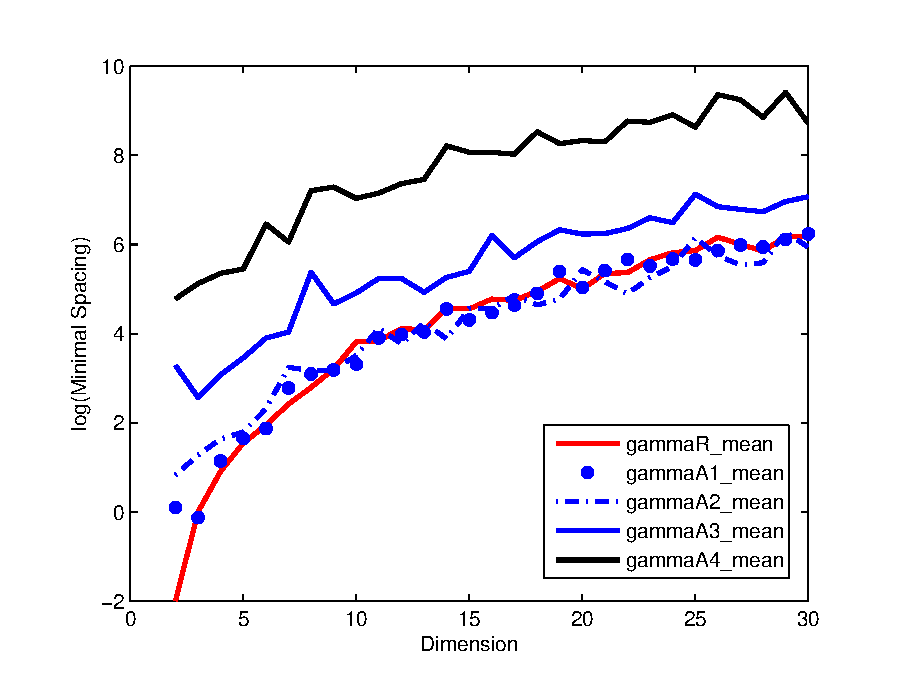
\includegraphics[width = 0.75\columnwidth]{miniSpacing}
\vspace{-0.4cm}
\caption{
\label{fig:miniSpacing}
 The values of $1/\gamma$ for matrices with different coherences}
\vspace{-0.5cm}
\end{figure}

\section{A Modified Version of DICA}
\label{subsec:modifiedDICA}
We would expect that DICA will achieve smaller error in the case of extreme coherence, since $1/\gamma_A$ will be much larger than $1/\gamma_R$. 
However, the experimental results in Section~\ref{subsubsec:results} show the opposite.  
The reason is that when the coherence is extremely high, the estimation
error of $M$ in DICA is so much larger than that in HKICA that it
dominates the error caused by the coherence of the mixing matrix.
This estimation error comes from taking the inverse of $T_2$ in DICA. 
Unfortunately, at the moment we don't understand well enough the relation of the estimation error and the coherence of the mixing matrix.

We propose the following ICA algorithm, Algorithm \ref{alg:DICA_Mod}, trying to relieve the estimation error problem of DICA, but still keeping the large gap of the eigenvalues in the eigen-decomposition. 
\begin{algorithm} 
\caption{DICA Modified (DICA\_Mod)}
\label{alg:DICA_Mod}
\begin{algorithmic}[1]
\INPUT $x(t)$ for $1\le t \le T$. 
\OUTPUT An estimation of the mixing matrix $A$. 
\STATE Sample $\psi$ from a $d$-dimensional standard Gaussian distribution;
\STATE Evaluate $\nabla^2\hat{f}(\psi)$, \\
%\quad where $\hat{m_p}(\eta) = \frac{1}{T}\sum_{k=1}^{T} (\eta^{\top}g(k))^p$, and $\hat{f}(\eta) = \frac{1}{12}\big(\hat{m_4}(\eta) - 3\hat{m_2}(\eta)^2 \big)$;
\STATE Compute $\hat{B}$ such that $\nabla^2\hat{f}(\psi) = \hat{B}\hat{B}^{\top}$;
\STATE Sample $\phi$ from the standard normal distribution;
\STATE Compute $\hat{T} = \nabla^2 \hat{f}(\hat{B}^{-\top}\phi)$;
\STATE Compute all the eigenvectors of $\hat{M} = \hat{B}^{-1}\hat{T}\hat{B}^{-\top}$, $\hat{R} = \{\mu_1,\ldots,\mu_d\}$;
\STATE Return $\hat{A} = \hat{B}\hat{R}$.
\end{algorithmic}
\end{algorithm}
\begin{remark}
\label{rmk:DICA_Mod}
Note that the eigenvalues of $\hat{M}$ in DICA\_Mod are $\frac{(\phi^{\top}R_i)^2}{(\psi^{\top}A_i)^4\kappa_i}$ for $1\le i\le d$. 
When $A$ is highly coherent, we would expect that $\psi^{\top}A_i$'s are close to each other. Also, the $\kappa_i$'s are fixed. 
Given that $\phi^{\top}R_i$'s are far separated from each other, we intuitively expect the eigenvalues to be well-separated from each other. 
However, we do not have a rigorous proof for this algorithm.
Experimental results show that DICA\_Mod consistently outperforms DICA. 
\end{remark}


\section{Proofs}
\label{sec:Appendix}

\subsection{Proof of Proposition \ref{prop:stochasticAss}}
Denote the population expectation by $\E$ and the empirical expectation by $\E_t$. We restate the assumptions here.
\begin{enumerate}[(i).]
\vspace{-3mm}
\item $\| \E_t[S] \|_F\le L/\sqrt{t}$;
\item $\| \E_t[\epsilon] \|_F \le L/\sqrt{t}$;
\item $\| \E_t[\epsilon^{\otimes 2}] \|_F \le L$;
\item $\| \E_t[\epsilon^{\otimes 3}] \|_F \le L$;
\item $\| \left(\E_{Y\sim \nu_t^{(\epsilon)}} [Y^{\otimes4}] - (\E_{Y\sim \nu_t^{(\epsilon)}} [Y^{\otimes2}])^{\otimes 2}\right)(\eta,\eta,\cdot,\cdot)  - 2 (\E_{Y\sim \nu_t^{(\epsilon)}} [Y^{\otimes2}])^{\otimes 2}(\eta,\cdot,\eta,\cdot)\|_F\le L/\sqrt{t} \|\eta\|_2^2$;
\item for $i_1,i_2,j_1,j_2 \ge 0$ that $i_1+i_2+j_1+j_2 \le 4$,  
\begin{align*}
\| \E_t[(AS)^{\otimes i_1} \otimes \E_t[\epsilon^{\otimes j_1}] \otimes (AS)^{\otimes i_2}] - \E_t[(AS)^{\otimes i_1}\otimes \epsilon^{\otimes j_1}\otimes (AS)^{\otimes i_2}]  \|_F \le L/\sqrt{t},
\end{align*}
and 
\begin{align*}
\| \E_t[\epsilon^{\otimes j_1} \otimes \E_t[(AS)^{\otimes i_1}] \otimes \epsilon^{\otimes j_2}] - \E_t[ \epsilon^{\otimes j_1}\otimes (AS)^{\otimes i_1}\otimes \epsilon^{\otimes j_2}]  \|_F \le L/\sqrt{t}.
\end{align*}
\end{enumerate}
Since $s$ is bounded by $C$, the first assumption will be satisfied with high probability $1-\delta$ by picking $L = C\sqrt{2d\log(\frac{1}{\delta})}$ by Hoeffding's inequality. Assumption (ii) to (v) are all about the moments of the Gaussian noise. 
For i.i.d. standard Gaussian random variables, $X_1, \ldots, X_t$, note that
\begin{itemize}
\item $ \E[\sum_j X_j/t] = 0$, $\text{Var}(\sum_j X_j/t) = 1/t$;
\item $ \E[\sum_j X_j^2/t] = 1$, $\text{Var}(\sum_j X_j^2/t) = 2/t$;
\item $ \E[\sum_j X_j^3/t] = 0$, $\text{Var}(\sum_j X_j^3/t) = 15/t$;
\item $ \E[\sum_j X_j^4/t] = 3$, $\text{Var}(\sum_j X_j^4/t) = 96/t$.
\end{itemize}
Therefore, by Chebyshev's inequality,
\begin{itemize}
\item with probability at least $1-\delta$, $|\sum_j X_j/t| \le \sqrt{1/t\delta}$;
\item with probability at least $1-\delta$, $|\sum_j X_j^2/t -1 | \le \sqrt{2/t\delta}$;
\item with probability at least $1-\delta$, $|\sum_j X_j^3/t| \le \sqrt{15/t\delta}$;
\item with probability at least $1-\delta$, $|\sum_j X_j^4/t -3| \le \sqrt{96/t\delta}$;
\end{itemize}
Given $\epsilon \sim \mathcal{N}(0,\Sigma)$ for some fixed unknown $\Sigma$, firstly consider the case when $\Sigma = I$.
Consider the $i$th entry of the 1-dimensional tensor (vector), with probability at least $1-\delta$, 
\[
\left| \sum_j \eps_i(j)/t \right| \le \sqrt{1/t\delta}.
\]
Thus, with probability at least $1-d\delta$,
\[
\| \sum_j \eps(j)/t \|_F \le \sqrt{d/t\delta}.
\]
For (iii), consider the position $(u,v)$ of the 2-dimensional tensor (matrix). If $u=v$ with probability at least $1-\delta$,
\[
	\left| \sum_j \eps_u^2(j)/t - 1\right| \le \sqrt{2/t\delta}.
\]
If $u\neq v$, by Chebysev's inequality with probability at least $1-\delta$,
\[
	\left| \sum_j \eps_u(j)\eps_v(j)/t \right| \le  \sqrt{1/t\delta}.
\]
Therefore, with probability at least $1-d^2\delta$, all entries are less that $1+\sqrt{2/t\delta}$. Thus 
\[
\|\E_t[\epsilon^{\otimes 2}]\|_F \le d(1+\sqrt{2/t\delta}).
\]
Similarly for (iv), consider the $(u,v,w)$ position for different cases. The expectation of $\eps_u\eps_v\eps_w$ is 0 and its variance is at most  $15$. Therefore, with probability at least $1-\delta$,
\[
\left|\sum_j \eps_u(j)\eps_v(j)\eps_w(j)/t \right| \le \sqrt{15/t\delta}.
\]
Thus, with probability at least $1-d^3\delta$,
\[
\|\E_t[\epsilon^{\otimes 3}]\|_F \le \sqrt{15d^3/t\delta}.
\] 
Lastly for (iv), each of the following inequalities holds with probability at least $1-\delta$,
\begin{align*}
& \left| \sum_j\eps_u^4(j)/t -3 \right| \le \sqrt{96/t\delta}; \quad \left| \sum_j\eps_u^3(j)\eps_v(j)/t \right| \le \sqrt{15/t\delta}; \quad \left| \sum_j\eps_u^2(j)\eps_v^2(j)/t - 1\right| \le \sqrt{4/t\delta}; \\
&  \left| \sum_j\eps_u^2(j)\eps_v(j)\eps_w(j)/t \right| \le \sqrt{2/t\delta}; \quad \left| \sum_j\eps_u(j)\eps_v(j)\eps_w(j)\eps_z(j)/t \right| \le \sqrt{1/t\delta};
\end{align*}
Consider the $(u,v)$ position of the matrix,
\begin{align*}
& \quad \left|\left(\E_t[\epsilon^{\otimes4}](\eta,\eta,\cdot,\cdot) - (\E_t[\epsilon^{\otimes2}])^{\otimes 2}(\eta,\eta,\cdot,\cdot) - 2(\E_t[\epsilon^{\otimes2}])^{\otimes 2}(\eta,\cdot,\eta,\cdot) \right)_{u,v}\right|\\
& \le \left| \left(\sum_j \eps_u(j)\eps_v(j)\sum_{k_1}\eta_{k_1}\eps_{k_1}(j)\sum_{k_2}\eta_{k_2}\eps_{k_2}(j)\right)/t- \E\left[ \eps_{u}\eps_{v}\sum_{k_1}\eta_{k_1}\eps_{k_1}\sum_{k_2}\eta_{k_2}\eps_{k_2}\right]\right| \\ 
& \quad + \left| \left(\sum_j \eps_u(j)\eps_v(j)\right)/t -  \E\left[ \eps_{u}\eps_{v}\right]\right|\left|\left(\sum_j\sum_{k_1}\eta_{k_1}\eps_{k_1}(j)\sum_{k_2}\eta_{k_2}\eps_{k_2}(j)\right)/t \right| \\
& \quad + 2\left| \left(\sum_j \eps_u(j)\sum_{k_1}\eta_{k_1}\eps_{k_1}(j)\right)/t\left(\sum_j \eps_v(j)\sum_{k_2}\eta_{k_2}\eps_{k_2}(j)\right)/t- \E\left[ \eps_{u}\sum_{k_1}\eta_{k_1}\eps_{k_1}\right]\E\left[\eps_{v}\sum_{k_2}\eta_{k_2}\eps_{k_2}\right]\right| 
\end{align*}
Note that the above inequality including $3d^2$ terms of concentration equations. Thus, with probability at least $1-3d^2\delta$,
\[
\left|\left(\E_t[\epsilon^{\otimes4}](\eta,\eta,\cdot,\cdot) - (\E_t[\epsilon^{\otimes2}])^{\otimes 2}(\eta,\eta,\cdot,\cdot) - 2(\E_t[\epsilon^{\otimes2}])^{\otimes 2}(\eta,\cdot,\eta,\cdot) \right)_{u,v}\right| 
\le
4\sqrt{15/t\delta}(1+\sqrt{2/t\delta})d\|\eta\|^2_2.  
\]
Thus, 
\[
\| \left(\E_{Y\sim \nu_t^{(\epsilon)}} [Y^{\otimes4}] - (\E_{Y\sim \nu_t^{(\epsilon)}} [Y^{\otimes2}])^{\otimes 2}\right)(\eta,\eta,\cdot,\cdot)  - 2 (\E_{Y\sim \nu_t^{(\epsilon)}} [Y^{\otimes2}])^{\otimes 2}(\eta,\cdot,\eta,\cdot)\|_F \le 4\sqrt{15/t\delta}(1+\sqrt{2/t\delta})d^2\|\eta\|^2_2.
\]
\if0
For the position $(i_1,i_2,i_3,i_4)$ of the tensor $\E_t[\epsilon^{\otimes4}] - 3(\E_t[\epsilon^{\otimes2}])^{\otimes 2}$ is
\[
\sum_j \eps_{i_1}(j)\eps_{i_2}(j)\eps_{i_3}(j)\eps_{i_4}(j)/t - 3(\sum_j \eps_{i_1}(j)\eps_{i_2}(j)/t)(\sum_j \eps_{i_3}(j)\eps_{i_4}(j)/t) = \sum_j \eps_i(t)^4/t - 3(\sum_j \eps_i(t)^2/t)^2  - \E[\eps_i^4] + 3(\E[\eps_i^2])^2.
\]  
Thus, 
\begin{align*}
|\sum_j \eps_i(t)^4/t - 3(\sum_j \eps_i(t)^2/t)^2| & \le \left|\sum_j \eps_i(t)^4/t - \E[\eps_i^4]\right| + \left|3(\sum_j \eps_i(t)^2/t)^2 - 3(\E[\eps_i^2])^2\right|. 
\end{align*}
Therefore, with probability at least $1-2\delta$, 
\[
|\sum_j \eps_i(t)^4/t - 3(\sum_j \eps_i(t)^2/t)^2| \le \sqrt{96/t\delta}+ 6(1+\sqrt{2/t\delta})\sqrt{2/t\delta}.
\]
Similarly, for the position $(i_1,i_1,i_1,i_2)$ (or its permutation), with probability at least $1-3\delta$,
\begin{align*}
&\quad |\sum_j \eps_{i_1}(t)^3\eps_{i_2}(t)/t - 3(\sum_j \eps_{i_1}(t)^2/t)(\sum_j \eps_{i_1}(t)\eps_{i_2}(t)/t)| \\
& \le \left|\sum_j \eps_{i_1}(t)^3\eps_{i_2}(t)/t -  \E[\eps_{i_1}^3 \eps_{i_2}]\right| +3\left|\sum_j \eps_{i_1}(t)^2/t\right|\left|\sum_j \eps_{i_1}(t)\eps_{i_2}(t)/t - \E[\eps_{i_1}\eps_{i_2}]\right| \\
& \le \sqrt{15/t\delta}+ 3(1+\sqrt{2/t\delta})\sqrt{1/t\delta}.
\end{align*}
Similarly, for the position $(i_1,i_1,i_2,i_2)$ (or its permutation), with probability at least $1-3\delta$,
\begin{align*}
&\quad |\sum_j \eps_{i_1}(t)^2\eps_{i_2}^2(t)/t - 3(\sum_j \eps_{i_1}(t)^2/t)(\sum_j \eps_{i_2}^2(t)/t)| \\
& \le \left|\sum_j \eps_{i_1}(t)^3\eps_{i_2}(t)/t -  \E[\eps_{i_1}^3 \eps_{i_2}]\right| +3\left|\sum_j \eps_{i_1}(t)^2/t\right|\left|\sum_j \eps_{i_1}(t)\eps_{i_2}(t)/t - \E[\eps_{i_1}\eps_{i_2}]\right| \\
& \le \sqrt{15/t\delta}+ 3(1+\sqrt{2/t\delta})\sqrt{1/t\delta}.
\end{align*}
Therefore, (ii) to (v) will be satisfied with probability $1-\delta$ by picking $L = \text{Poly}(\|\Sigma\|_{(\infty,\infty)}, d)\sqrt{\log(\frac{1}{\delta})}$ for some polynomial $\text{Poly}(\cdot)$.
\fi
For the last assumption, since the Gaussian noise $\epsilon$ is independent to the source signals $s$, by triangular inequality 
\begin{align*}
&\|\E_t[(AS)^{\otimes i_1}\otimes \E_t[\epsilon^{\otimes j_1}] \otimes (AS)^{\otimes i_2}] - \E_t[(AS)^{\otimes i_1}\otimes \epsilon^{\otimes j_1}\otimes (AS)^{\otimes i_2}]  \|_F \\
& \quad \le  \|\E_t[(AS)^{\otimes i_1}\otimes \E_t[\epsilon^{\otimes j_1}] \otimes (AS)^{\otimes i_2}] - \E_t[(AS)^{\otimes i_1}\otimes \E[\epsilon^{\otimes j_1}] \otimes (AS)^{\otimes i_2}] \|_F \\
& \quad \quad + \| \E_t[(AS)^{\otimes i_1}\otimes \E[\epsilon^{\otimes j_1}] \otimes (AS)^{\otimes i_2}] - \E[(AS)^{\otimes i_1}\otimes \E[\epsilon^{\otimes j_1}] \otimes (AS)^{\otimes i_2}] \|_F \\
& \quad \quad + \underbrace{\|\E[(AS)^{\otimes i_1}\otimes \E[\epsilon^{\otimes j_1}] \otimes (AS)^{\otimes i_2}]  - \E[(AS)^{\otimes i_1}\otimes \epsilon^{\otimes j_1}\otimes (AS)^{\otimes i_2}] \|_F}_{=0} \\
& \quad \quad + \| \E[(AS)^{\otimes i_1}\otimes \epsilon^{\otimes j_1}\otimes (AS)^{\otimes i_2}] - \E_t[(AS)^{\otimes i_1}\otimes \epsilon^{\otimes j_1}\otimes (AS)^{\otimes i_2}] \|_F.
\end{align*}
Note that every term in the RHS is a concentration inequality of $i_1+j_1+i_2$-dimensional tensors. Similarly we can consider each position of these tensors which has finite variance.
Thus, with probability at least $1- 4d^{(i_1+j_1+i_2)}\delta$,   
\[
\|\E_t[(AS)^{\otimes i_1}\otimes \E_t[\epsilon^{\otimes j_1}] \otimes (AS)^{\otimes i_2}] - \E_t[(AS)^{\otimes i_1}\otimes \epsilon^{\otimes j_1}\otimes (AS)^{\otimes i_2}]  \|_F 
\le
12(1+\sqrt{2/t\delta})d^{(i_1+j_1+i_2)/2}A_{\max}^{i_1+i_2}C^{i_1+i_2}\sqrt{96/t\delta}.  
\]
Similar argument will go through for the second inequality.
Therefore, there exists $\hat{L} = \text{Poly}(\frac{1}{\delta}, A_{\max}, C, d)$, such that for probability at least $1-\delta$, the above conclusions hold simultaneously.

Lastly, for general case where $\eps\sim {\cN}(0,\Sigma)$, the above conclusions will apply for $\Sigma^{-1/2}\eps$. Thus picking $L = \|\Sigma\|^4_2\hat{L}$, all bounds will still hold. 
\subsection{Limit Effect of the Noise} 
\label{subsec:denoise}
\begin{prop}
 Suppose Assumptions~\ref{ass:gauss} and~\ref{ass:independence} hold. Then,
for any vector $\eta$ satisfying $\|\eta\|_2\le L_{\eta}$,
\[
\| \nabla^2f_{\nu_T^{(x)}}(\eta) - \nabla^2f_{\nu_T^{(As)}}(\eta) \|_2 \le \frac{\poly{L_{\eta}, L, d, \sigma_{\max}(A), C}}{\sqrt{T}}. 
\] 
\end{prop}
Note that 
\begin{align*}
& \E_{(X,Y)\sim \nu_T^{(s,\epsilon)}} [(AX+Y)^{\otimes 4}]\\
 = & \,\E_{X\sim \nu_T^{(s)}}[(AX)^{\otimes 4}] \\
& \quad+ \E_{(X,Y)\sim \nu_T^{(s,\epsilon)}} [(AX)^{\otimes 3}\otimes Y + (AX)^{\otimes 2}\otimes Y\otimes (AX) + (AX)\otimes Y\otimes (AX)^{\otimes 2} + Y\otimes (AX)^{\otimes 3}] \\
& \quad+ E_{(X,Y)\sim \nu_T^{(s,\epsilon)}} [ (AX)^{\otimes 2}\otimes Y^{\otimes 2} + (AX)\otimes Y\otimes (AX)\otimes Y + (AX)\otimes Y^{\otimes 2}\otimes (AX)]\\
& \quad+  E_{(X,Y)\sim \nu_T^{(s,\epsilon)}} [ (Y)^{\otimes 2}\otimes (AX)^{\otimes 2} + (Y)\otimes (AX)\otimes Y\otimes (AX) + Y\otimes (AX)^{\otimes 2}\otimes Y] \\
& \quad+ E_{(X,Y)\sim \nu_T^{(s,\epsilon)}} [Y^{\otimes 3}\otimes (AX) + Y^{\otimes 2}\otimes (AX)\otimes Y + Y\otimes (AX)\otimes Y^{\otimes 2} + (AX)\otimes Y^{\otimes 3}] \\
& \quad+ \E_{Y\sim \nu_T^{(\epsilon)}}[Y^{\otimes 4}].
\end{align*}
We can bound
\begin{align*}
& \| \E_{(X,Y)\sim \nu_T^{(s,\epsilon)}} [(AX)^{\otimes 3}\otimes Y + (AX)^{\otimes 2}\otimes Y\otimes (AX) + (AX)\otimes Y\otimes (AX)^{\otimes 2} + Y\otimes (AX)^{\otimes 3}] \|_F \\
\le \,& \,  \| \E_{X\sim \nu_T^{(s)}} [(AX)^{\otimes 3}] \otimes \E_{Y\sim \nu_T^{(\epsilon)}}[Y] + \E_{X\sim \nu_T^{(s)}} [(AX)^{\otimes 2} \otimes \E_{Y\sim \nu_T^{(\epsilon)}}[Y] \otimes (AX)] \\
& \quad + \E_{X\sim \nu_T^{(s)}} [(AX) \otimes \E_{Y\sim \nu_T^{(\epsilon)}}[Y] \otimes (AX)^{\otimes 2}]  + \E_{Y\sim \nu_T^{(\epsilon)}}[Y] \otimes \E_{X\sim \nu_T^{(s)}} [(AX)^{\otimes 3}] \|_F + \frac{4L}{\sqrt{T}} \\
\le \, & \,\frac{4L(d^{3/2}\sigma^3_{\max}(A)C^3 +1)}{\sqrt{T}},
\end{align*}
and similarly, 
\[
\| E_{(X,Y)\sim \nu_T^{(s,\epsilon)}} [Y^{\otimes 3}\otimes (AX) + Y^{\otimes 2}\otimes (AX)\otimes Y + Y\otimes (AX)\otimes Y^{\otimes 2} + (AX)\otimes Y^{\otimes 3}] \|_F \le \frac{4L(L+1)}{\sqrt{T}}.
\]
Combining these two terms together, we have 
\begin{align*}
& \E_{(X,Y)\sim \nu_T^{(s,\epsilon)}} [(AX+Y)^{\otimes 4}]\\
 = & \,\E_{X\sim \nu_T^{(s)}}[(AX)^{\otimes 4}] + \E_{Y\sim \nu_T^{(\epsilon)}}[Y^{\otimes 4}] + K_1 +K_2,
\end{align*}
where $\|K_1\|_F \le\frac{\text{Poly}(L, d, \sigma_{\max}(A), C)}{\sqrt{T}} $, and 
\begin{align*}
K2  = & E_{(X,Y)\sim \nu_T^{(s,\epsilon)}} [ (AX)^{\otimes 2}\otimes Y^{\otimes 2} + (AX)\otimes Y\otimes (AX)\otimes Y + (AX)\otimes Y^{\otimes 2}\otimes (AX)]\\
& \quad+  E_{(X,Y)\sim \nu_T^{(s,\epsilon)}} [ (Y)^{\otimes 2}\otimes (AX)^{\otimes 2} + (Y)\otimes (AX)\otimes Y\otimes (AX) + Y\otimes (AX)^{\otimes 2}\otimes Y]. 
\end{align*}
A similar computation can be applied to $\E_{(X,Y)\sim \nu_t^{(s,\epsilon)}} [(AX+Y)^{\otimes 2}]$.
\begin{align*}
\E_{(X,Y)\sim \nu_t^{(s,\epsilon)}} [(AX+Y)^{\otimes 2}]= & \, \E_{X\sim \nu_t^{(s)}}[(AX)^{\otimes 2}] + \E_{(X,Y)\sim \nu_t^{(s,\epsilon)}}[(AX)\otimes Y + Y\otimes (AX)] + \E_{Y\sim \nu_t^{(\epsilon)}}[Y^{\otimes 2}].
\end{align*}
Then again,
\[
\|\E_{(X,Y)\sim \nu_t^{(s,\epsilon)}}[(AX)\otimes Y + Y\otimes (AX)]\|_F \le \frac{2L(L+1)}{\sqrt{T}}.
\]
Thus, 
\[
\left( \E_{(X,Y)\sim \nu_t^{(s,\epsilon)}} [(AX+Y)^{\otimes 2}]\right)^{\otimes2} =  \left(\E_{X\sim \nu_t^{(s)}}[(AX)^{\otimes 2}]\right)^{\otimes2} + \left( \E_{Y\sim \nu_t^{(\epsilon)}}[Y^{\otimes 2}]\right)^{\otimes 2} + K_3+K_4,
\]
where $\|K_3\|_F \le \frac{\text{Poly}(L, d, \sigma_{\max}, C)}{\sqrt{T}}$, and $K_4 = \E_{X\sim \nu_t^{(s)}}[(AX)^{\otimes 2}] \otimes \E_{Y\sim \nu_t^{(\epsilon)}}[Y^{\otimes 2}] + \E_{Y\sim \nu_t^{(\epsilon)}}[Y^{\otimes 2}] \otimes \E_{X\sim \nu_t^{(s)}}[(AX)^{\otimes 2}]$.

Note that $\nabla^2f_{\nu_T^{(x)}}(\eta)$ and $\nabla^2f_{\nu_T^{(As)}}(\eta)$ are the matrices generated by marginalizing 2 dimensions of the tensors on the direction $\eta$:  
\begin{align*}
\nabla^2f_{\nu_T^{(x)}}(\eta) =\, &\, \E_{(X,Y)\sim \nu_T^{(s,\epsilon)}} [(AX+Y)^{\otimes 4}](\eta,\eta,\cdot,\cdot) - \left( \E_{(X,Y)\sim \nu_T^{(s,\epsilon)}} [(AX+Y)^{\otimes 2}]\right)^2 (\eta,\eta,\cdot,\cdot) \\
& \quad - 2\left( \E_{(X,Y)\sim \nu_T^{(s,\epsilon)}} [(AX+Y)^{\otimes 2}]\right)^2 (\eta,\cdot,\eta,\cdot).
\end{align*}
Similarly, 
\begin{align*}
\nabla^2f_{\nu_T^{(As)}}(\eta) = & \E_{X\sim \nu_T^{(s)}}[(AX)^{\otimes 4}](\eta,\eta,\cdot,\cdot) - \left(\E_{X\sim \nu_T^{(s)}}[(AX)^{\otimes 2}]\right)^2(\eta,\eta,\cdot,\cdot) \\
& \quad - 2 \left(\E_{X\sim \nu_T^{(s)}}[(AX)^{\otimes 2}]\right)^2(\eta,\cdot,\eta,\cdot). 
\end{align*}
Also note that $\| \left[\E_{Y\sim \nu_t^{(\epsilon)}}[Y^{\otimes 4}] - 3\left(\E_{Y\sim \nu_t^{(\epsilon)}}[Y^{\otimes 2}]\right)^{\otimes 2} \right]\|_F \le \frac{L}{\sqrt{t}}$.
Therefore,
\begin{align*}
%\label{eq:HessionApprox1}
\|\nabla^2f_{\nu_T^{(x)}}(\eta) -  \nabla^2f_{\nu_T^{(As)}}(\eta) \|_F \le & \|K_1(\eta,\eta,\cdot, \cdot)\|_F + \|(K_2-K_4)(\eta,\eta,\cdot, \cdot) - 2K_4(\eta,\cdot,\eta,\cdot)\|_F + 3 \|K_3(\eta,\eta,\cdot, \cdot)\|_F + \frac{L}{\sqrt{T}}\\
\le & \|(K_2-K_4)(\eta,\eta,\cdot, \cdot) - 2K_4(\eta,\cdot,\eta,\cdot)\|_F + \frac{\text{Poly}(L_{\eta}, L, d, \sigma_{\max}, C)}{\sqrt{T}}.
\end{align*}

It remains to bound $\|(K_2-K_4)(\eta,\eta,\cdot, \cdot) - 2K_4(\eta,\cdot,\eta,\cdot)\|_F$. 
Note that $E_{(X,Y)\sim \nu_T^{(s,\epsilon)}} [ (AX)\otimes Y\otimes (AX)\otimes Y](\eta,\eta,\cdot,\cdot)  = E_{(X,Y)\sim \nu_T^{(s,\epsilon)}} [ (AX)^{\otimes 2}\otimes Y^{\otimes 2}](\eta,\cdot,\eta,\cdot)$.
\begin{align*}
& \|(K_2-K_4)(\eta,\eta,\cdot, \cdot) - 2K_4(\eta,\cdot,\eta,\cdot)\|_F \\
\le\,  & \,\|\left( E_{(X,Y)\sim \nu_T^{(s,\epsilon)}} [ (AX)^{\otimes 2}\otimes Y^{\otimes 2}]- \E_{X\sim \nu_t^{(s)}}[(AX)^{\otimes 2}] \otimes \E_{Y\sim \nu_t^{(\epsilon)}}[Y^{\otimes 2}]\right)(\eta,\eta,\cdot,\cdot)\|_F \\
& \quad + \|\left( E_{(X,Y)\sim \nu_T^{(s,\epsilon)}} [ Y^{\otimes 2}\otimes (AX)^{\otimes 2}]- \E_{Y\sim \nu_t^{(\epsilon)}}[Y^{\otimes 2}] \otimes \E_{X\sim \nu_t^{(s)}}[(AX)^{\otimes 2}]\right)(\eta,\eta,\cdot,\cdot)\|_F \\
& \quad + 2\|\left( E_{(X,Y)\sim \nu_T^{(s,\epsilon)}} [ (AX)^{\otimes 2}\otimes Y^{\otimes 2}]- \E_{X\sim \nu_t^{(s)}}[(AX)^{\otimes 2}] \otimes \E_{Y\sim \nu_t^{(\epsilon)}}[Y^{\otimes 2}]\right)(\eta,\cdot,\eta,\cdot)\|_F \\
& \quad + \|\left( E_{(X,Y)\sim \nu_T^{(s,\epsilon)}} [ Y^{\otimes 2}\otimes (AX)^{\otimes 2}]- \E_{Y\sim \nu_t^{(\epsilon)}}[Y^{\otimes 2}] \otimes \E_{X\sim \nu_t^{(s)}}[(AX)^{\otimes 2}]\right)(\eta,\cdot,\eta, \cdot)\|_F \\
\le \, &\, \frac{\text{Poly}(L_{\eta}, L, d, \sigma_{\max}, C)}{\sqrt{T}}. 
\end{align*}
Combining the above two inequalities leads to the conclusion.


\subsection{Proof of Theorem \ref{thm:efficiency}}
\label{subsec:ProofEfficiency}
The following result is proven by \citet{hsu2013learning}:
\begin{thm}[\citet{hsu2013learning}, Theorem~4]
Assume $A$ is nonsingular. 
Let $m_4,m_2:\real^d \ra \real$ be defined by Equation \eqref{eq:momnent} with respect to the product distribution $\mu$,
	while $f_{\mu}: \real^d \ra \real$ be defined by Equation \eqref{eq:funcf}.
Let $\phi,\psi\in \real^d$ be vectors from the unit sphere of $\real^d$. Then, 
	the matrix
\begin{equation}
\label{eq:M}
M =(\nabla^2f_{\mu}(\phi))(\nabla^2f_{\mu}(\psi))^{-1} 
\end{equation}
can be written in the diagonal form
\begin{equation}
\label{eq:M2}
M = A 
\left(
\begin{array}{ccc}
\lambda_1 & & \\ %\left(\frac{\phi^{\top}A_1}{\psi^{\top}A_1}\right)^2 & &\\
    & \ddots & \\
    & & \lambda_d %\left(\frac{\phi^{\top}A_d}{\psi^{\top}A_d}\right)^2\\
\end{array} 
\right) 
A^{-1},
\end{equation}
where $\lambda_i = \left(\frac{\phi^{\top}A_i}{\psi^{\top}A_i}\right)^2$.
\end{thm}

It follows from this theorem that 
if $\phi,\psi$ are chosen independently from the uniform distribution on the unit sphere of $\real^d$, with probability one,
the eigenvalues of  $M$ are all distinct and the corresponding eigenvectors
determine the rows of $A$ up to permutation and scaling.
%Now since we have a product measure $\mu$ that $\nu_T^{(s)}$ is close to, we can treat $s(t)$ is an empirical instance from the distribution $\mu$.  

The following lemma bounds $\|\nabla^2 f_{\mu}(\eta) - \nabla^2 \hat{f}(\eta) \|_2$ by $\xi$:
\begin{lemma}
\label{lem:nablavariation}
\[
\|\nabla^2 f_{\mu}(A^{\top}\eta) - \nabla^2 \hat{f_{\nu_T^{(As)}}}(\eta)  \|_2 \le \|\nabla^2 f_{\mu}(\eta) - \nabla^2 \hat{f_{\nu_T^{(As)}}}(\eta)  \|_F\le  \|\eta\|_2^2  d^5 A_{(2,\max)}^2A_{\max}^2\xi.
\]
Thus, 
\[
\|\nabla^2 f_{\mu}(A^{\top}\eta) - \nabla^2\hat{f}(\eta)\|_2 \le  \|\eta\|_2^2  d^5 A_{(2,\max)}^2A_{\max}^2\xi + P(\|\eta\|_2).
\]
\end{lemma}
\begin{proof}
Without loss of generality assume $\|\eta\|_2 = 1$.
Note that  
\[
\nabla^2 f_{A^{\top}\mu}(\eta) = G_1(\eta) - G_2(\eta) -2G_3(\eta),
\]
and 
\[
\nabla^2 \hat{f}_{\nu_T^{(As)}}(\eta) =\hat{G_1}(\eta) - \hat{G_2}(\eta) -2\hat{G_3}(\eta),
\]
where 
\begin{align*}
& G_1(\eta) = \int (\eta^{\top}As)^2Ass^{\top}A^{\top}\,d\mu(s); \\
& G_2(\eta) = \int (\eta^{\top}As)^2\,d\mu(s) \int Ass^{\top}A^{\top} \,d\mu(s); \\
& G_3(\eta) = \Big(\int (\eta^{\top}As)As\,d\mu(s)\Big)\Big(\int (\eta^{\top}As)As\,d\mu(s)\Big)^{\top}. \\
&\hat{ G_1}(\eta) = \frac1n\sum_{k=1}^{n} \big(\eta^{\top}As(k)\big)^2As(k)s(k)^{\top}A^{\top} = \int (\eta^{\top}As)^2Ass^{\top}A^{\top}\,d\nu_T(s); \\
& \hat{G_2}(\eta) = \frac{1}{n^2}\sum_{k=1}^{n} \big(\eta^{\top}As(k)\big)^2 \sum_{k=1}^{n}As(k)s(k)^{\top}A^{\top} = \int (\eta^{\top}As)^2\,d\nu_T(s) \int Ass^{\top}A^{\top} \,d\nu_T(s); \\
& \hat{G_3}(\eta) = \frac{1}{n^2}\Big(\sum_{k=1}^{n} \big(\eta^{\top}As(k)\big)As(k)\Big) \Big(\sum_{k=1}^{n} \big(\eta^{\top}As(k)\big)As(k)\Big)^{\top} = \Big(\int (\eta^{\top}As)As\,d\nu_T(s)\Big)\Big(\int (\eta^{\top}As)As\,d\nu_T(s)\Big)^{\top}.
\end{align*}

%Without loss of generality, assume $ \|\eta\|_2 = 1$.
Note that all the integral functions of $G_i(\eta)$ or $\hat{G_i}(\eta)$ are matrices of polynomials in $x$. Thus, we only need to bound its coefficients.
%Also, since $|b_1b_2b_3b_4| \le \frac14(b_1^4+b_2^4+b_3^4+b_4^4)$, we only need to upper bound the coefficients of $x_i^4$. 
Note that 
\[
\left(G_1\right)_{i,j} = \int (\sum_t \eta^{\top}A_ts_t)^2\sum_t A_{i,t}s_t \sum_t A_{j,t}s_t d\mu(s).
\]
Thus, the coefficient of the term $s_{t_1}s_{t_2}s_{t_3}s_{t_4}$ is $\eta^{\top}A_{t_1}\eta^{\top}A_{t_2}A_{i,t_3}A_{j,t_4}$, 
which is bounded by $\max_i |\eta^{\top} A_i|^2 A_{\max}^2 \le A_{(2,\max)}^2A_{\max}^2$. 
Thus,
\[
\left| (G_1)_{i,j} - (\hat{G_1})_{i,j} \right| \le d^4  A_{(2,\max)}^2A_{\max}^2D_4(\mu, \nu_T).
\]

Similarly, 
\[
\left| \int A_{i:}ss^{\top}A_{j:}^{\top} \,d\mu(s) - \int A_{i:}ss^{\top}A_{j:}^{\top} \,d\nu_T(s) \right| \le d^2 A_{\max}^2 D_2(\mu,\nu_T)
\]
 and 
\[
\left| \int (\eta^{\top}As)^2\,d\mu(s) -\int (\eta^{\top}As)^2\,d\nu_T(s) \right| \le d^2 A_{(2,\max)}^2 D_2(\mu,\nu_T).
\]
Also note that $ \left| \int (\eta^{\top}As)^2\,d\mu(s) \right| \le d^2A_{(2,\max)}^2 C^2$, and
$\left| \int A_{i:}ss^{\top}A_{j:}^{\top} \,d\nu_T(s) \right| \le d^2A_{\max}^2 C^2$.
Now consider the difference between $G_2$ and $\hat{G_2}$. 
\begin{align*}
& \left| (G_2)_{i,j} - (\hat{G_2})_{i,j} \right| \\
=\, & \left| \int (\eta^{\top}As)^2\,d\mu(s) \int A_{i:}ss^{\top}A_{j:}^{\top} \,d\mu(s)  - 
\int (\eta^{\top}As)^2\,d\nu_T(s) \int A_{i:}ss^{\top}A_{j:}^{\top} \,d\nu_T(s) \right| \\
\le \, & \left| \int (\eta^{\top}As)^2\,d\mu(s) \int A_{i:}ss^{\top}A_{j:}^{\top} \,d\mu(s)  - 
\int (\eta^{\top}As)^2\,d\mu(s) \int A_{i:}ss^{\top}A_{j:}^{\top} \,d\nu_T(s) \right| \\ 
& \quad + \left| \int (\eta^{\top}As)^2\,d\mu(s) \int A_{i:}ss^{\top}A_{j:}^{\top} \,d\nu_T(s)  - 
\int (\eta^{\top}As)^2\,d\nu_T(s) \int A_{i:}ss^{\top}A_{j:}^{\top} \,d\nu_T(s) \right| \\
\le\, & \left| \int (\eta^{\top}As)^2\,d\mu(s) \right| \left|\int A_{i:}ss^{\top}A_{j:}^{\top} \,d\mu(s) - \int A_{i:}ss^{\top}A_{j:}^{\top} \,d\nu_T(s) \right| \\
& \quad + \left| \int (\eta^{\top}As)^2\,d\mu(s) -\int (\eta^{\top}As)^2\,d\nu_T(s) \right| \left| \int A_{i:}ss^{\top}A_{j:}^{\top} \,d\nu_T(s) \right| \\
\le\, & 2 d^4  A_{(2,\max)}^2A_{\max}^2C^2D_2(\mu, \nu_T).
\end{align*}
Similarly,
\[
\left| (G_3)_{i,j} - (\hat{G_3})_{i,j} \right| \le 2 d^4  A_{(2,\max)}^2A_{\max}^2C^2D_2(\mu, \nu_T).
\]
Thus for any $1\le i,j\le d$,
\begin{align*}
\left|\left(\nabla^2 f_{\mu}(A^{\top}\eta) \right)_{i,j} - \left(\nabla^2 \hat{f}_{\nu_T^{(As)}}(\eta) \right)_{i,j} \right| 
\le 
d^4  A_{(2,\max)}^2A_{\max}^2\left( 6C^2D_2(\mu, \nu_T) + D_4(\mu, \nu_T)\right).
\end{align*}
Therefore, 
\[
\|\nabla^2 f_{\mu}(A^{\top}\eta) - \nabla^2 \hat{f}_{\nu_T^{(As)}}(\eta)  \|_2 \le \|\nabla^2 f_{\mu}(A^{\top}\eta) - \nabla^2 \hat{f}_{\nu_T^{(As)}}(\eta) \|_F \le d^5  A_{(2,\max)}^2A_{\max}^2\left( 6C^2D_2(\mu, \nu_T) + D_4(\mu, \nu_T)\right).
\]
Lastly, combining with Proposition \ref{prop:denoise}, 
\[
\|\nabla^2 f_{\mu}(A^{\top}\eta) - \nabla^2\hat{f}(\eta)\|_2 \le \|\nabla^2 f_{\mu}(A^{\top}\eta) - \nabla^2 \hat{f}_{\nu_T^{(As)}}(\eta)\|_2 + \| \nabla^2 \hat{f}_{\nu_T^{(As)}}(\eta) - \nabla^2\hat{f}(\eta)\|_2 \le \|\eta\|_2^2  d^5 A_{(2,\max)}^2A_{\max}^2\xi + P(\|\eta\|_2).
\]
\end{proof}
Before we can prove the theorem, we need to prove some lemmas.
The following lemma shows that a small perturbation of $M$ will only result in a small variation of its eigenvectors, at least under some mild regularity conditions.
\begin{lemma}
\label{lem:eigenvectorvariation}
Denote $\hat{M} = M+E$ be a perturbation of matrix $M$, where $M$ is defined in  \eqref{eq:M2}. 
Assume $\hat{M}$ has distinct eigenvalues. 
If $\gamma_A > 4 \frac{\sigma_{\max}(A)}{\sigma_{\min}(A)}\|E\|_2$, and $\min_{i,j:i\neq j} \|A_i - A_j\|_2 > \frac{8}{\gamma_A}\frac{\sigma_{\max}^2(A)}{\sigma_{\min}(A) } \|E\|_2$, then there exist a permutation $\pi$ and constants $\{c_1,\ldots,c_d\}$, such that 
\[
\max_{1\le k\le d} \| c_1\hat{A}_{\pi(k)} - A_k\|_2 \le 4  \frac{\sigma_{\max}^2(A)}{\gamma_A \sigma_{\min}(A) } \|E\|_2\,,
\]
and therefore
\[
\sum_{k=1}^{d}\| c_1\hat{A}_{\pi(k)} - A_k\|_2 \le 4d  \frac{\sigma_{\max}^2(A)}{\gamma_A \sigma_{\min}(A)} \|E\|_2\,,
\]
where $\hat{A}$ is the matrix of eigenvectors of $\hat{M}$. 
\end{lemma}
\begin{proof}
For $1\le k\le d$, assume 
\[
A_{(k)}^{-1} E A_{(k)} =  
\left(
\begin{array}{cc}
F_{1k} & F_{2k}\\
F_{3k} & F_{4k} \\
\end{array} 
\right), 
\]
where $A_{(k)}$ is the matrix $(A_k, A_1, \cdots, A_{k-1}, A_{k+1}, \cdots, A_d)$.
Let $\gamma_k = \|F_{3k}\|_2$, $\eta_k = \|F_{2k}\|_2$, and 
\[
\delta_k = \min_{j: j\neq k} 
\left\vert \left(\frac{\phi^{\top}A_k}{\psi^{\top}A_k}\right)^2 -\left( \frac{\phi^{\top}A_j}{\psi^{\top}A_j}\right)^2 \right\vert - \|F_{1k}\|_2 - \|F_{4k}\|_2\,.
\]
Note that by definition, $\gamma_k = \|F_{3k}\|_2\le\|A_{(k)}^{-1}EA_{k}\|_2\le\frac{\sigma_{\max}(A)}{\sigma_{\min}(A)}\|E\|_2$,
 $\eta_k = \|F_{2k}\|_2\le\|(A^{-1})_kEA_{(k)}\|_2\le\frac{\sigma_{\max}(A)}{\sigma_{\min}(A)}\|E\|_2$, 
 and $\|F_{1k}\|_2,\|F_{4k}\|_2\le\|A_{(k)}^{-1} E A_{(k)}\|_2\le\frac{\sigma_{\max}(A)}{\sigma_{\min}(A)}\|E\|_2$. 
 Thus,
\begin{align*}
\delta_k & = \min_{j:j\neq k} 
	\left\vert \left(\frac{\phi^{\top}A_k}{\psi^{\top}A_k}\right)^2 - \left(\frac{\phi^{\top}A_j}{\psi^{\top}A_j}\right)^2 \right\vert - \|F_{1k}\|_2 - \|F_{4k}\|_2\\
	& \ge \min_{j:j\neq k} \left\vert \left(\frac{\phi^{\top}A_k}{\psi^{\top}A_k}\right)^2 - \left(\frac{\phi^{\top}A_j}{\psi^{\top}A_j}\right)^2 \right\vert - 2 \frac{\sigma_{\max}(A)}{\sigma_{\min}(A)}\|E\|_2\\
	& \ge  \gamma_A -  2 \frac{\sigma_{\max}(A)}{\sigma_{\min}(A)}\|E\|_2 \\
	& >  2 \frac{\sigma_{\max}(A)}{\sigma_{\min}(A)}\|E\|_2 >0,
\end{align*}
and $\delta_k^2 > 4\gamma_k\eta_k$. 
Therefore, by Theorem 2.8, Chapter V of \citep{stewart1990matrix}, there exist a unique vector $v$ satisfying $\|v\|_2\le 2\frac{\gamma_k}{\delta_k}$ such that there exists one of a eigenvector $\hat{A_k}$ of $\hat{M}$ satisfying
 \[
 \|\hat{A_k} - A_k\|_2 \le \|A_{ck}\|_2 \|v\|_2 \le 2\sigma_{\max}(A)\frac{\gamma_k}{\delta_k}
 \le 
 \frac{4\sigma_{\max}^2(A)}{\gamma_A \sigma_{\min}(A) } \|E\|_2,
 \]
 where $A_{ck}$ is the $d\times (d-1)$ matrix $(A_1,\ldots,A_{k-1}, A_{k+1},\ldots,A_d)$.
 By condition, for $i\neq j$,  $\frac{8\sigma_{\max}^2(A)}{\gamma_A \sigma_{\min}(A) } \|E\|_2 < \|A_i - A_j\|_2\le \|A_i - \hat{A_i}\|_2 + \|A_j - \hat{A_i}\|_2$, thus $\hat{A_i} \neq \hat{A_j}$.  Summing up the upper bound gets the result. 
\end{proof}
The next lemma shows that $\hat{X}^{-1}$ is close to $X^{-1}$ with respect to  matrix induced $2$-norm.
\begin{lemma}
\label{lem:inversevariation}
If non-singular matrix $\hat{X} = X+E$ satisfying that $\sigma_{\min}(X)\ge2\|E\|_2$, then $\|\hat{X}^{-1}\|_2 \le \frac{2}{\sigma_{\min}(X)}$, and $\|\hat{X}^{-1} - X^{-1} \|_2 \le \frac{2}{\sigma_{\min}^2(X)}\|E\|_2$.
\end{lemma} 
\begin{proof}
Note that $\|\hat{X}^{-1}\|_2$ is the inverse of the minimal singular value of $\hat{X}$. Also, 
\[
 \min_{v:\|v\|_2=1} \|\hat{X}v\|_2 = \min_{v:\|v\|_2=1}\|(X+E)v\|_2 \ge \min_{v:\|v\|_2=1} \|Xv\|_2 - \|Ev\|_2 \ge \sigma_{\min}(X) - \|E\|_2.
\]
So $\|\hat{X}^{-1}\|_2 \le \frac{1}{\sigma_{\min}(X) - \|E\|_2} \le \frac{2}{\sigma_{\min}(X)}$. Moreover,
\begin{align*}
\|\hat{X}^{-1} - X^{-1} \|_2 \le \|X^{-1}\|_2\|\hat{X}^{-1}\|_2\|\hat{X} - X\|_2
\le \frac{2}{\sigma_{\min}^2(X)}\|E\|_2.
\end{align*}
\end{proof}
Now we can estimate the variance between $XY^{-1}$ and $(X+E_1)(Y+E_2)^{-1}$.
\begin{lemma}
\label{lem:Mvariation}
Assume that $\sigma_{\min}(Y)\ge2\|E_2\|_2$, then
\[
\| XY^{-1} - (X+E_1)(Y+E_2)^{-1}\|_2 \le \frac{2\|X\|_2}{\sigma_{\min}^2(Y)}\|E_2\|_2 + \frac{2}{\sigma_{\min}(Y)}\|E_1\|_2.
\]
\end{lemma}
\begin{proof}
Applying Lemma \ref{lem:inversevariation},
\begin{align*}
	& \| XY^{-1} - (X+E_1)(Y+E_2)^{-1}\|_2 \\
\le\, & \| XY^{-1} - X(Y+E_2)^{-1}\|_2 + \| X(Y+E_2)^{-1} - (X+E_1)(Y+E_2)^{-1}\|_2 \\
\le\, & \|X\|_2\| Y^{-1} - (Y+E_2)^{-1}\|_2 + \|E_1\|_2\|(Y+E_2)^{-1}\|_2\\
\le\, & \frac{2\|X\|_2}{\sigma_{\min}^2(Y)}\|E_2\|_2 + \frac{2}{\sigma_{\min}(Y)}\|E_1\|_2
\end{align*}
\end{proof}


Note that $\nabla^2f_{\mu}(\psi) = \sum_{i=1}^{d} \kappa_i(\psi^{\top}A_i)^2A_iA_i^{\top} = AKD_{\psi}A^{\top}$,  where $D_{\psi} = \text{diag}\left((\psi^{\top}A_1)^2,\cdots, (\psi^{\top}A_d)^2\right)$ (see, e.g., \citealt{hsu2013learning}). 
Thus, $\sigma_{\min}(\nabla^2f_{\mu}(\psi)) = \min_{v:\|v\|_2=1}\|\sum_{i=1}^{d} \kappa_i(\psi^{\top}A_i)^2A_iA_i^{\top}v\|_2$. 
\begin{lemma}
\label{lem:boundsigmaminnabla}
On the event $\Epsi$, $\sigma_{\max}(\nabla^2f_{\mu}(\psi)) \le L_u^2 \kappa_{\max}A^2_{(2,\max)}\sigma_{\max}^2(A)$, and
 $\sigma_{\min}(\nabla^2f_{\mu}(\psi)) \ge \frac{\sqrt{2\pi}}{2d} \ell^2\kappa_{\min}A^2_{(2,\min)}\sigma_{\min}^2(A)$.
\end{lemma}
\begin{proof}
Note that $\nabla^2f_{\mu}(\psi)$ is symmetric. 
For any unit vector $v$, $v^{\top}AD_{\psi}KA^{\top}v \ge \frac{\sqrt{2\pi}}{2d}\ell^2\kappa_{\min} A^2_{(2,\min)}\|v^{\top}A\|_2^2 \ge \frac{\sqrt{2\pi}}{2d}\ell^2\kappa_{\min}A^2_{(2,\min)}\sigma_{\min}^2(A)$. Similar calculation for the maximum singular value.
\end{proof}

Lastly, we still need to bound $\|M - \hat{M}\|_2$.
\begin{lemma}
\label{lem:Mvariation_alg}
Given that  $\xi \le  \frac{\sqrt{2\pi}\kappa_{\min}A^2_{(2,\min)}\sigma_{\min}^2(A)\ell^2}{8L_u^2d^6 A_{(2,\max)}^2A_{\max}^2}$ and $T$  is large enough, but still polynomial in $\{L_\eta, C, \sigma_{\max}(A), L\}$, such that $P(L_u) \le \frac{\sqrt{2\pi}}{8d}\kappa_{\min}A^2_{(2,\min)}\sigma_{\min}^2(A)\ell^2$, then on the event $\Epsi$, 
\[ 
\|M - \hat{M}\|_2 \le 2\left( \frac{2L_u^2d^2A_{(2,\max)}^2\kappa_{\max}\sigma_{\max}^2(A)}{\pi\kappa^2_{\min}A^4_{(2,\min)}\sigma_{\min}^4(A)\ell^4} + 
\frac{\sqrt{2}d}{\sqrt{\pi}\kappa_{\min}A^2_{(2,\min)}\sigma_{\min}^2(A)\ell^2}
\right)\left(L_u^2d^5 A_{(2,\max)}^2A_{\max}^2\xi + P(L_u)\right).
\]
\end{lemma}
\begin{proof}
Let $E_1 = \nabla^2 f_{\mu}(\phi) - \nabla^2 \hat{f}(\phi)$ and $ E_2 = \nabla^2 f_{\mu}(\psi) - \nabla^2 \hat{f}(\psi)$. Then $\|E_1\|_2 , \|E_2\|_2 \le L_u^2d^5 A_{(2,\max)}^2A_{\max}^2\xi + P$.
Note $\nabla^2f(\phi) = AKD_{\phi} A^{\top}$.
Given that 
$\xi \le  \frac{\sqrt{2\pi}\kappa_{\min}A^2_{(2,\min)}\sigma_{\min}^2(A)\ell^2}{8L_u^2d^6 A_{(2,\max)}^2A_{\max}^2}$ 
and $P(L_u) \le \frac{\sqrt{2\pi}}{8d}\kappa_{\min}A^2_{(2,\min)}\sigma_{\min}^2(A)\ell^2$, the condition in Lemma \ref{lem:Mvariation} holds on the event $\Epsi$. 
Then apply Lemma \ref{lem:Mvariation} and \ref{lem:nablavariation}, we have
\begin{align*}
\|M - \hat{M}\|_2 =\, & \|(\nabla^2 f(\phi))(\nabla^2f(\psi))^{-1} - (\nabla^2 \hat{f}(\phi))(\nabla^2\hat{f}(\psi))^{-1} \|_2 \\
\le \, &\frac{2\|\nabla^2 f(\phi)\|_2}{\sigma_{\min}^2(\nabla^2f(\psi))}\|E_2\|_2 + \frac{2}{\sigma_{\min}(\nabla^2f(\psi))}\|E_1\|_2 \\
\le \, & 2\left( \frac{2L_u^2d^2A_{(2,\max)}^2\kappa_{\max}\sigma_{\max}^2(A)}{\pi\kappa^2_{\min}A^4_{(2,\min)}\sigma_{\min}^4(A)\ell^4} + 
\frac{\sqrt{2}d}{\sqrt{\pi}\kappa_{\min}A^2_{(2,\min)}\sigma_{\min}^2(A)\ell^2}
\right)\left(L_u^2d^5 A_{(2,\max)}^2A_{\max}^2\xi + P(L_u)\right).
\end{align*}
\if0
Thus, 
\[ 
\|M - \hat{M}\|_2 \le \frac{4d^7A_{(2,\max)}^4A_{\max}^2\kappa_{\max}\sigma_{\max}^2(A) + 2\sqrt{2\pi}d^6A_{(2,\max)}^2A_{\max}^2\kappa_{\min}A^2_{(2,\min)}\sigma_{\min}^2(A)}{\pi\kappa^2_{\min}A^4_{(2,\min)}\sigma_{\min}^4(A)} \xi.
\]
\fi
\end{proof}
\begin{proof}[{\bf Proof of Theorem  \ref{thm:efficiency}}]
Let 
 \begin{align*}
Q = 2\left( \frac{2L_u^2d^2A_{(2,\max)}^2\kappa_{\max}\sigma_{\max}^2(A)}{\pi\kappa^2_{\min}A^4_{(2,\min)}\sigma_{\min}^4(A)\ell^4} + 
\frac{\sqrt{2}d}{\sqrt{\pi}\kappa_{\min}A^2_{(2,\min)}\sigma_{\min}^2(A)\ell^2}
\right)\left(L_u^2d^5 A_{(2,\max)}^2A_{\max}^2\xi + P(L_u)\right)
 \end{align*}
 where $\xi$ is defined in Equation \eqref{eq:xi}.
 Note that $P(L_u)$ is proportional to $1/\sqrt{T}$, thus given large enough $T$ and small enough $\xi$, the following conditions hold:
 \begin{enumerate}
 \vspace{-3mm}
 \item $\gamma_A > 4\frac{\sigma_{\max}(A)}{\sigma_{\min}(A)} Q$
 \item $\min_{i,j:i\neq j} \|A_i - A_j\|_2 > \frac{8}{\gamma_A}\frac{\sigma_{\max}^2(A)}{\sigma_{\min}(A) } Q$;
 \item $\xi \le \frac{\sqrt{2\pi}\kappa_{\min}A^2_{(2,\min)}\sigma_{\min}^2(A)\ell^2}{8L_u^2d^6 A_{(2,\max)}^2A_{\max}^2}$;
 \item  $P(L_u) \le \frac{\sqrt{2\pi}}{8d}\ell^2\kappa_{\min}A^2_{(2,\min)}\sigma_{\min}^2(A)$. 
  \end{enumerate}

Note that $M = \nabla^2f(\phi))(\nabla^2f(\psi))^{-1}$ and $\hat{M}$ has distinct eigen-values with probability 1,  then by Lemma \ref{lem:Mvariation_alg}, $\|M-\hat{M}\|_2 \le Q$.
Therefore, by lemma \ref{lem:eigenvectorvariation}, 
  \[
  \max_{1\le k\le d}\| c_1\hat{A}_{\pi(k)} - A_k\|_2 \le 4 \frac{\sigma_{\max}^2(A)}{\gamma_A \sigma_{\min}(A)}\|M - \hat{M} \|_2 \le 4 \frac{\sigma_{\max}^2(A)}{\gamma_A \sigma_{\min}(A)} Q. 
  \]
 %and 
 %\[
 %\sum_{k=1}^{d}\| c_1\hat{A}_{\pi(k)} - A_k\|_2 \le 4d\frac{\sigma_{\max}^2(A)}{\gamma_A \sigma_{\min}(A)}\|M - \hat{M} \|_2. 
% \]
 
\end{proof}

\subsection{Analysis of DICA -- Proof of Theorem~\ref{thm:finalRes}}
\label{subsec:ProofModEff}

Let 
\begin{align*}
\bar{\xi} &=   \frac{\sqrt{2}d\left(L_u^2d^5 A_{(2,\max)}^2A_{\max}^2\xi + P\right)}{\sqrt{\pi}\ell^2\kappa_{\min}A^2_{(2,\min)}\sigma_{\min}^2(A)}, \\
\hat{\xi} &= \frac{3L_u^2d^5A^2_{\max}}{2\kappa_{\min}C_1^2}\xi + \frac{\sqrt{6}L_u^2\sigma_{\max}^2(A)}{C_1^2}\bar{\xi}, \\
 Q &=  
 %\frac{32\sqrt{2}d^5\kappa^{3/2}_{\max}A^6_{(2,\max)}}{\pi^{5/2}\kappa_{\min}A^4_{(2,\min)}} \sqrt{\hat{\xi}}.
 \frac{4L_u^2A^6_{(2,\max)}}{l_l^4 A^6_{(2,\min)}}\left(\hat{\xi}
 +
 P\left(\frac{\sqrt{3}L_u}{\sqrt{2}\sigma_{\min}(A)\kappa_{\min}^{1/2}C_1}\right)\right).
\end{align*} 
%Similar to Lemma~\ref{lem:dmin}, on the event $\Ephi$ with probability at least $1/4$, $\text{min}_i |\phi_1^{\top}R_i| \ge \frac{\sqrt{2\pi}}{2d}$ (respectively $\text{min}_i |\phi_2^{\top}R_i| \ge \frac{\sqrt{2\pi}}{2d}$). 
%Denote this event by $\Ephione$ (respectively $\Ephitwo$).

First we start with proving the following theorem:
\begin{thm}
\label{thm:Modefficiency}
 Assume the following conditions hold:
 \begin{enumerate}
 \vspace{-3mm}
 \item $\hat{T}$ has distinct eigenvalues;
 \item $\gamma_R > 4 \frac{\sigma_{\max}^2(A)}{\sigma_{\min}(A) }Q$; 
 \item $\min_{i,j:i\neq j} \|A_i - A_j\|_2 > \frac{8}{\gamma_R}\frac{\sigma_{\max}^2(A)}{\sigma_{\min}(A) } Q$;
 \item $\xi \le \frac{\sqrt{\pi}\kappa_{\min}A^2_{(2,\min)}\sigma_{\min}^2(A)}{6\sqrt{2}d^6A_{(2,\max)}^2A_{\max}^2}$
 \item $P(L_u) \le \frac{\sqrt{\pi}\ell^2\kappa_{\min}A^2_{(2,\min)}\sigma_{\min}^2(A)}{6\sqrt{2}d}$
 (so $\bar{\xi} \le 1/3$);
 \item $\hat{\xi}
  +
  P\left(\frac{\sqrt{3}L_u}{\sqrt{2}\sigma_{\min}(A)\kappa_{\min}^{1/2}C_1}\right) \le \frac{l_l^2 A^2_{(2,\min)}}{2A^2_{(2,\max)}}$.
 \end{enumerate}
 \vspace{-2mm}
Then on the event $\Epsi \cap\Ephi$, there exists a permutation $\pi$ and constants $\{c_1,\ldots,c_d\}$, such that for $1\le k\le d$,
\[
%\|c_k\hat{R}_{\pi(k)} - (R^*R)_k\|_2 \le \frac{4}{\gamma_R} \|\hat{T} - T\|_2\,,
\| c_k\hat{A}_{\pi(k)} - A_k\|_2 \le \frac{4\sigma^2_{\max}(A)}{\gamma_R\sigma_{\min}(A)} Q,
\]
where $\hat{A}$ is the output of the DICA algorithm.
\end{thm}

Note that $\nabla^2f_{\mu}(\psi) = AKD_{\psi}A^{\top}$. Thus $B = AK^{1/2}D_{\psi}^{1/2}R^{\top}$ for some orthonormal matrix $R$. 
We need to introduce some lemmas before we can prove the theorem. 
The following lemma shows the stability of the square root of matrix.
\begin{lemma}
\label{lem:matrixsquareroot}
Given two symmetric matrices $X$ and $\hat{X} = X + E$, where $X = HH^{\top}$ and $\hat{X} = \hat{H}\hat{H}^{\top}$, such that $\|X^{-1}\|_2 \|E\|_2 < 1$, then every singular value of $H^{-1}\hat{H}$ is bounded between $\sqrt{1- \|X^{-1}\|_2 \|E\|_2}$ and $\sqrt{1+ \|X^{-1}\|_2 \|E\|_2}$, 
and every singular value of $\hat{H}^{-1}H$ is bounded between $\frac{1}{\sqrt{1 + \|X^{-1}\|_2 \|E\|_2}}$ and $\frac{1}{\sqrt{1 - \|X^{-1}\|_2 \|E\|_2}}$. 
\end{lemma}
\begin{proof}
For any unit vector $x$,
\begin{align*}
& x^{\top}H^{-1}\hat{H}\hat{H}^{\top}H^{-\top}x - x^{\top}x\\
& \quad = x^{\top}H^{-1}\left( \hat{H}\hat{H}^{\top} - HH^{\top}\right)H^{-\top}x \\
& \quad \le \|H^{-\top}x\|^2_2 \|E\|_2 \\
& \quad \le \|X^{-1}\|_2^2 \|E\|_2.
\end{align*}
Thus every singular value of $H^{-1}\hat{H}$ is bounded between $\sqrt{1- \|X^{-1}\|_2 \|E\|_2}$ and $\sqrt{1+ \|X^{-1}\|_2 \|E\|_2}$, 
and every singular value of $\hat{H}^{-1}H$ is bounded between $\frac{1}{\sqrt{1 + \|X^{-1}\|_2 \|E\|_2}}$ and $\frac{1}{\sqrt{1 - \|X^{-1}\|_2 \|E\|_2}}$.
\end{proof}
Applying Lemma \ref{lem:matrixsquareroot}, we can get the stability of $B$, as follows.
\begin{lemma}
\label{lem:BhatinverseB}
Given that $\xi \le \frac{\sqrt{\pi}\kappa_{\min}A^2_{(2,\min)}\sigma_{\min}^2(A)}{6\sqrt{2}L_u^2d^6A_{(2,\max)}^2A_{\max}^2}$ and $P(L_u)\le \frac{\sqrt{\pi}\ell^2\kappa_{\min}A^2_{(2,\min)}\sigma_{\min}^2(A)}{6\sqrt{2}d}$
(so $\bar{\xi} \le 1/3$), under the event $\Epsi$ there exists an orthonormal matrix $R^*$ such that 
 \[
 \sqrt{1-\bar{\xi}} \le \|B^{-1}\hat{B}\|_2 \le \sqrt{1+\bar{\xi}},
 \]
 and
\[
\|\hat{B}^{-1}B - R^*\|_2 \le \bar{\xi}.
\]
\end{lemma}
\begin{proof}
Note that by Lemma \ref{lem:boundsigmaminnabla},  under the event $\Epsi$, $\|\nabla^2f(\psi)\|_2 \ge \frac{\sqrt{2\pi}}{2d}\ell^2\kappa_{\min}A^2_{(2,\min)}\sigma_{\min}^2(A)$. Thus,
\[
\|\left(\nabla^2f(\psi)\right)^{-1}\|_2 \|E\|_2 \le \frac{\sqrt{2}d}{\sqrt{\pi}\ell^2\kappa_{\min}A^2_{(2,\min)}\sigma_{\min}^2(A)}\left(L_u^2d^5 A_{(2,\max)}^2A_{\max}^2\xi + P(L_u)\right) = \bar{\xi}.
\]
Then given $\xi \le \frac{\sqrt{\pi}\kappa_{\min}A^2_{(2,\min)}\sigma_{\min}^2(A)}{6\sqrt{2}L_u^2d^6A_{(2,\max)}^2A_{\max}^2}$
and 
$P(L_u) \le \frac{\sqrt{\pi}\ell^2\kappa_{\min}A^2_{(2,\min)}\sigma_{\min}^2(A)}{6\sqrt{2}d}$, $\bar{\xi} \le 1/3 < 1$. 
By Lemma \ref{lem:matrixsquareroot}, every singular value of $\hat{B}^{-1}B$ is bounded between $\frac{1}{\sqrt{1 + \|\left(\nabla^2f(\psi)\right)^{-1}\|_2 \|E\|_2}}$ and $\frac{1}{\sqrt{1 - \|\left(\nabla^2f(\psi)\right)^{-1}\|_2 \|E\|_2}}$. 
Thus every singular value of $\hat{B}^{-1}B$ is bounded between $\frac{1}{\sqrt{1+\bar{\xi}}}$ and $\frac{1}{\sqrt{1-\bar{\xi}}}$, i.e. there exist an orthonormal matrix $R^*$ such that 
\[
\|\hat{B}^{-1}B - R^*\|_2 \le \max \left\{ \left|1-\frac{1}{\sqrt{1+\bar{\xi}}}\right| , \left|\frac{1}{\sqrt{1-\bar{\xi}}}-1\right| \right\} \le \bar{\xi},
\]
where the last inequality is by $\bar{\xi} \le 1/3$.
\end{proof}

Define $T_i$ by $T_i = G(B^{-\top}{R^*}^{\top}\phi_i) = A D_{\psi}^{-1}\Lambda_iA^{\top}$ for $i \in \{1,2\}$,
where $\Lambda_i = \text{diag}\left((\phi_i^{\top}R^*R_1)^2, \cdots, (\phi_i^{\top}R^*R_d)^2\right)$. 
Then, 
\begin{equation}
\label{eq:T}
M = A \Lambda_1 \Lambda_2^{-1} A^{-1} = A \Lambda A^{-1},
\end{equation}
where $\Lambda = \text{diag}\left((\frac{\phi_1^{\top}R^*R_1}{\phi_2^{\top}R^*R_1})^2, \cdots, (\frac{\phi_1^{\top}R^*R_d}{\phi_2^{\top}R^*R_d})^2\right)$. 

Similarly, we have the stability of the eigen-decomposition, as follows. 
\begin{lemma}
\label{lem:Teigenvectorvariation}
Denote $\hat{M} = M+E$ be a perturbation of matrix $M$, where $M$ is defined in Equation \eqref{eq:T}. 
Assume $\hat{T}$ has distinct eigenvalues. 
If $\gamma_R > 4 \frac{\sigma_{\max}^2(A)}{\sigma_{\min}(A) }\|E\|_2$ and $\min_{i,j:i\neq j} \|A_i - A_j\|_2 > \frac{8}{\gamma_R}\frac{\sigma_{\max}^2(A)}{\sigma_{\min}(A) } \|E\|_2$, then there exist a permutation $\pi$ and constants $\{c_1,\ldots,c_d\}$, such that for $1\le k\le d$
\[
\| c_k\hat{A}_{\pi(k)} - A_k\|_2 \le \frac{4\sigma^2_{\max}(A)}{\gamma_R\sigma_{\min}(A)} \|E\|_2\,,
\]
where $\hat{A}$ is the matrix of eigenvectors of $\hat{M}$. 
\end{lemma}
\begin{proof}
The proof is similar to that of Lemma \ref{lem:eigenvectorvariation}.
\end{proof}
It still remains to bound $\|E\|_2$. In the event $\Ephi$, we take the orthogonal matrix $\tilde{R}$ as $R^*R$ in Equation \ref{eq:T} for the remaining of this paper.

\begin{lemma}
\label{lem:Binversenablavariation1}
Given that $\xi \le \frac{\sqrt{\pi}\kappa_{\min}A^2_{(2,\min)}\sigma_{\min}^2(A)}{6\sqrt{2}d^6A_{(2,\max)}^2A_{\max}^2}$ and $P(L_u) \le \frac{\sqrt{\pi}\ell^2\kappa_{\min}A^2_{(2,\min)}\sigma_{\min}^2(A)}{6\sqrt{2}d}$
(so $\bar{\xi} \le 1/3$), then on the event $\Epsi$ and $\Ephi$ for $\phi \in \{\phi_1, \phi_2\}$,
\[
\|\nabla^2 f_{\mu}(A^{\top}B^{-\top}{R^*}^{\top}\phi) - \nabla^2 \hat{f}_{\nu_T^{(As)}}(\hat{B}^{-\top}\phi)  \|_2 
= \|G(B^{-\top}{R^*}^{\top}\phi) - \hat{G}(\hat{B}^{-\top}\phi)\|_2
\le 
\frac{3L_u^2d^5A^2_{\max}}{2\kappa_{\min}C_1^2}\xi + \frac{\sqrt{6}L_u^2\sigma_{\max}^2(A)}{C_1^2}\bar{\xi}
\le \hat{\xi}.
\]
\end{lemma}
\begin{proof}
Note that by Lemma \ref{lem:nablavariation} $\|\nabla^2 f(\psi) - \nabla^2 \hat{f}(\psi)\|_2 \le L_u^2  d^5 A_{(2,\max)}^2A_{\max}^2\xi$, and 
\[
\|G(B^{-\top}R{^*}^{\top}\phi) - \hat{G}(\hat{B}^{-\top}\phi)\|_2
\le 
\|G(B^{-\top}{R^*}^{\top}\phi) - G(\hat{B}^{-\top}\phi)\|_2
+ \|G(\hat{B}^{-\top}\phi) - \hat{G}(\hat{B}^{-\top}\phi)\|_2.
\]

To Bound $\|G(\hat{B}^{-\top}\phi) - \hat{G}(\hat{B}^{-\top}\phi)\|_2$, we will need the following properties which are straightforward based on Lemma \ref{lem:BhatinverseB}: 
under the event $ \Epsi\cap \Ephi $ for $1\le i, j\le d$,
\begin{itemize}
\item $|\phi^{\top}\hat{B}^{-1}A_i| \le \|\phi\|_2\|\hat{B}^{-1}B\|_2\|B^{-1}A_i\|_2\le
 \frac{L_u}{\sqrt{1-\bar{\xi}}} (K^{-1/2}D^{-1/2}_{\psi})_{ii} \le
 \frac{L_u}{\sqrt{1-\bar{\xi}}\kappa_{\min}^{1/2}C_1}$.
\end{itemize}
Thus for $1\le i, j\le d$,
\[
|(G_1(\hat{B}^{-\top}\phi))_{i,j} - (\hat{G_1}(\hat{B}^{-\top}\phi))_{i,j}| \le
d^4A^2_{\max}\frac{L_u^2}{(1-\bar{\xi})\kappa_{\min}C_1^2}D_4(\nu,\nu_t).
\]
Also note that for $1\le i, j\le d$,
\begin{itemize}
\item $|\int(\phi^{\top}\hat{B}^{-1}x)x_i d\Prob{s}| 
\le L_u\int \|\hat{B}^{-1}A\|_2\|s\|_2 |A_{i:}s| d\Prob{s}
\le \frac{L_ud^{3/2}C^2A_{\max}}{\sqrt{1-\bar{\xi}}\kappa_{\min}^{1/2}C_1}$; 
\item $|(\hat{B}^{-1}A)_{ij}| \le \frac{1}{\sqrt{1-\bar{\xi}}\kappa_{\min}^{1/2}C_1}$;
\item $|\int(\phi^{\top}\hat{B}^{-1}x)^2 d\Prob{s}|\le
 \int \|\phi\|_2^2 \|\hat{B}^{-1}A\|_2^2\|s\|_2^2 d\Prob{s} \le \frac{L_u^2dC^2}{(1-\bar{\xi})\kappa_{\min}C_1^2}$.
\end{itemize}
Thus, similar to \ref{lem:nablavariation},
\[
|(G_2(\hat{B}^{-\top}\phi))_{i,j} - (\hat{G_2}(\hat{B}^{-\top}\phi))_{i,j}| \le
\frac{2L_u^2d^3C^2A^2_{\max}}{(1-\bar{\xi})\kappa_{\min}C_1^2}D_2(\nu,\nu_t),
\]
and 
\[
|(G_3(\hat{B}^{-\top}\phi))_{i,j} - (\hat{G_3}(\hat{B}^{-\top}\phi))_{i,j}| \le
\frac{2L_u^2d^{7/2}C^2A^2_{\max}}{(1-\bar{\xi})\kappa_{\min}C_1^2}D_2(\nu,\nu_t).
\]
Therefore for $1\le i,j\le d$,
\[
\left|\left(G(\hat{B}^{-\top}\phi)\right)_{i,j} - \left(\hat{G}(\hat{B}^{-\top}\phi)\right)_{i,j}\right| 
\le
\frac{L_u^2d^4A^2_{\max}}{(1-\bar{\xi})\kappa_{\min}C_1^2}D_2(\nu,\nu_t). 
\]
Thus, 
\begin{equation}
\label{eq:fBhatfhatBhat}
 \|G(\hat{B}^{-\top}\phi) - \hat{G}(\hat{B}^{-\top}\phi)\|_2 \le 
\frac{3L_u^2d^5A^2_{\max}}{2\kappa_{\min}C_1^2}\xi.
\end{equation}

On the other hand, 
\begin{align*}
\|G(B^{-\top}{R^*}^{\top}\phi_i) - G(\hat{B}^{-\top}\phi_i)\|_2 
= & \, \|A D_{\psi}^{-1}\Lambda_iA^{\top}- A D_{\psi}^{-1}\hat{\Lambda}_iA^{\top}\|_2 \\
\le & \, \|A\|^2_2 \|D_{\psi}^{-1}\|_2 \|\Lambda_i - \hat{\Lambda}_i\|_2\\
\le & \, 2\frac{\sigma_{\max}^2(A)}{C_1^2}\frac{L_u^2\bar{\xi}}{\sqrt{1-\bar{\xi}}},
\end{align*}
where $\hat{\Lambda}_i = \text{diag}\left((\phi_i^{\top}\hat{B}^{-1}BR_1)^2, \cdots, (\phi_i^{\top}\hat{B}^{-1}BR_d)^2\right)$.
Thus,
\begin{equation}
\label{eq:fBfBhat}
\|G(B^{-\top}{R^*}^{\top}\phi) - G(\hat{B}^{-\top}\phi)\|_2 \le  \frac{\sqrt{6}L_u^2\sigma_{\max}^2(A)}{C_1^2}\bar{\xi}. 
\end{equation}

Combine Equation \eqref{eq:fBhatfhatBhat} and Equation \eqref{eq:fBfBhat},
\[
\|G(B^{-\top}{R^*}^{\top}\phi) - \hat{G}(\hat{B}^{-\top}\phi)\|_2
\le 
\frac{3L_u^2d^5A^2_{\max}}{2\kappa_{\min}C_1^2}\xi + \frac{\sqrt{6}L_u^2\sigma_{\max}^2(A)}{C_1^2}\bar{\xi}.
\]
\end{proof}

\begin{lemma}
\label{lem:Binversenablavariation2}
Given the same conditions as Lemma \ref{lem:BhatinverseB}, then on the event $\Epsi$ and $\Ephi$ for $\phi \in \{\phi_1, \phi_2\}$,
\[
\|\nabla^2 f_{\mu}(A^{\top}B^{-\top}{R^*}^{\top}\phi) - \nabla^2 \hat{f}_{\nu_T^{(As)}}(\hat{B}^{-\top}\phi)  \|_2 
\le
 \hat{\xi}
+
\frac{1}{T}\text{Poly}\left(\frac{1}{\sigma_{\min}(A)}, \frac{1}{C_1}, L_u, \frac{1}{\kappa_{\min}}, L, d, \sigma_{\max}(A), C\right).
\]
\end{lemma}
\begin{proof}
By triangular inequality, 
\[
\|\nabla^2 f_{\mu}(A^{\top}B^{-\top}{R^*}^{\top}\phi) - \nabla^2 \hat{f}(\hat{B}^{-\top}\phi)  \|_2 
\le 
\|\nabla^2 f_{\mu}(A^{\top}B^{-\top}{R^*}^{\top}\phi) - \nabla^2 \hat{f}_{\nu_T^{(As)}}(\hat{B}^{-\top}\phi)  \|_2 
+
\|\nabla^2 \hat{f}_{\nu_T^{(As)}}(\hat{B}^{-\top}\phi) - \nabla^2 \hat{f}(\hat{B}^{-\top}\phi)  \|_2. 
\]
By Lemma \ref{lem:Binversenablavariation1}, 
\[
\|\nabla^2 f_{\mu}(A^{\top}B^{-\top}{R^*}^{\top}\phi) - \nabla^2 \hat{f}_{\nu_T^{(As)}}(\hat{B}^{-\top}\phi)  \|_2 
\le \hat{\xi}. 
\]
It remains to bound the second term. 
Note that on the event $\Epsi\cap\Ephi$, $\|\hat{B}^{-\top}\phi\|_2 \le \frac{\sqrt{3}L_u}{\sqrt{2}\sigma_{\min}(A)\kappa_{\min}^{1/2}C_1}$. 
Thus by Proposition \ref{prop:denoise}, 
\[
\|\nabla^2 \hat{f}_{\nu_T^{(As)}}(\hat{B}^{-\top}\phi) - \nabla^2 \hat{f}(\hat{B}^{-\top}\phi)  \|_2 \le P\left(\frac{\sqrt{3}L_u}{\sqrt{2}\sigma_{\min}(A)\kappa_{\min}^{1/2}C_1}\right).
\]
Therefore, 
\[
\|\nabla^2 f_{\mu}(A^{\top}B^{-\top}{R^*}^{\top}\phi) - \nabla^2 \hat{f}(\hat{B}^{-\top}\phi)  \|_2 
\le 
 \hat{\xi}
+
P\left(\frac{\sqrt{3}L_u}{\sqrt{2}\sigma_{\min}(A)\kappa_{\min}^{1/2}C_1}\right).
\]
\end{proof}
\begin{lemma}
\label{lem:Tvariantion}
Given the same conditions as Lemma \ref{lem:BhatinverseB}, On the event $\Epsi$ and $\Ephi$, assume that $\hat{\xi}
+
P\left(\frac{\sqrt{3}L_u}{\sqrt{2}\sigma_{\min}(A)\kappa_{\min}^{1/2}C_1}\right)\le \frac{l_l^2 A^2_{(2,\min)}}{2A^2_{(2,\max)}}$, then 
\[
\|M - \hat{M}\|_2 \le  \frac{128d^6A^6_{(2,\max)}}{\pi^3 A^6_{(2,\min)}}\left(\hat{\xi}+
P\left(\frac{\sqrt{3}L_u}{\sqrt{2}\sigma_{\min}(A)\kappa_{\min}^{1/2}C_1}\right)\right) = Q.
\]
\end{lemma}

\begin{proof}
On the event $\Epsi\cap\Ephi$,
\[
\sigma_{\min}(T_2) \ge \frac{l_l^2A^2_{(2,\min)}}{A^2_{(2,\max)}}; \quad \sigma_{\max}(T_2) \le \frac{L_u^2A^2_{(2,\max)}}{A^2_{(2,\min)}};  \quad \sigma_{\max}(T_1) \le \frac{L_u^2A^2_{(2,\max)}}{A^2_{(2,\min)}}. 
\]
Let $E_i = \nabla^2 f_{\mu}(A^{\top}B^{-\top}{R^*}^{\top}\phi_i) - \nabla^2 \hat{f}(\hat{B}^{-\top}\phi_i)$ for  $i\in\{1,2\}$. then by 
Lemma \ref{lem:Binversenablavariation1} $\sigma_{\min}(T_2) \ge 2\|E_2\|_2$.
Apply Lemma \ref{lem:Mvariation},
\begin{align*}
\|M - \hat{M}\|_2 \le &
\frac{2\|T_1\|_2}{\sigma^2_{\min}(T_2)}\|E_2\|_2 + \frac{2}{\sigma_{\min}(T_2)}\|E_1\|_2 \\
\le & \frac{4L_u^2A^6_{(2,\max)}}{l_l^4 A^6_{(2,\min)}}\left(\hat{\xi}
+
P\left(\frac{\sqrt{3}L_u}{\sqrt{2}\sigma_{\min}(A)\kappa_{\min}^{1/2}C_1}\right)\right) = Q.
\end{align*}
\end{proof}
\begin{proof}[{\bf Proof of Theorem \ref{thm:Modefficiency}}]
Note that by Lemma \ref{lem:Tvariantion},
\[
\|\hat{M} - M\|_2 \le Q.
\]
Then by Lemma \ref{lem:Teigenvectorvariation}, there exists a permutation $\pi$ and constants $\{c_1,\ldots,c_d\}$, such that for $1\le k\le d$,
\[
\| c_k\hat{A}_{\pi(k)} - A_k\|_2 \le \frac{4\sigma^2_{\max}(A)}{\gamma_R\sigma_{\min}(A)} \|\hat{M} - M\|_2.
\]
\end{proof}

Before finishing the proof of Theorem \ref{thm:finalRes}, we need another auxiliary result, whose proof is deferred to Section~\ref{sec:events}:
\begin{lemma}
\label{lem:ConstantProb}
With Probability at least $1-\delta$ , the following inequalities holds simultaneously.
\begin{itemize}
\vspace{-3mm}
\item $\min_i |\psi^{\top}A_i| \ge \frac{\sqrt{\pi}A_{(2,\min)}}{5\sqrt{2}(d+1)} \delta$;
\item $\min_i \{|\phi_2^{\top}R_i|\} \ge \frac{\sqrt{\pi}}{5\sqrt{2}(d+1)}\delta$;
\item $\|\phi_1\|_2, \|\phi_2\|_2 \le \sqrt{2}\left(\sqrt{\log(\frac{5}{\delta})}+\sqrt{d}\right)$;
\item $\gamma_R \ge\frac{\delta}{2d^2}$.
\end{itemize}
\vspace{-2mm}
\end{lemma}
Denote the above event by $\E$.
\begin{remark}
Note that all the constants in Lemma~\ref{lem:ConstantProb} are polynomial in $d$ (or $d^{-1}$ for the lower bound), thus the result of Theorem~\ref{thm:Modefficiency} is polynomial in $d$ and $\frac{1}{\delta}$ with probability at least $1-\delta$. \qed
\end{remark}

\subsubsection{Proof of Theorem \ref{thm:finalRes}}
We need to verify the validness of the conditions of Theorem~\ref{thm:Modefficiency} in the traditional stochastic setting. 
Note that the first condition holds with probability 1. 
The other 5 conditions can be satisfied by small enough 
$\hat{\xi}$, small enough $\bar{\xi}$, small enough $P(L_u)$, and small enough $P\left(\frac{\sqrt{3}L_u}{\sqrt{2}\sigma_{\min}(A)\kappa_{\min}^{1/2}C_1}\right)$.
By Proposition~\ref{prop:denoise}, $P(L_u)$ and $P\left(\frac{\sqrt{3}L_u}{\sqrt{2}\sigma_{\min}(A)\kappa_{\min}^{1/2}C_1}\right)$ can be arbitrarily small given large enough sample size 
\[T = \poly{d.\frac{1}{\kappa_{\min}}, \frac{1}{\sigma_{\min}(A)}, \frac{1}{\ell}, L_u, L, C, \sigma_{\max}(A)}.\] 
$\hat{\xi}$ and $\bar{\xi}$ will be small if $\xi$ is small enough.
Recall Equation \eqref{eq:xi} that 
\[\xi = \left( 6C^2D_2(\mu, \nu_T) + D_4(\mu, \nu_T)\right) \le 7C^2D_4(\mu, \nu_T),\]
where $C$ is an upper bound for the signal function $s$.
%\[\xi = \poly{\frac{1}{L_u}, \frac{\sigma_{\min}(A)}{\sigma_{\max}(A)}, \ell, \gamma_R, \frac{1}{\sigma_{\max}(A)},\frac{1}{d}, \kappa_{\min}\sigma_{\min}^4(A)}.\] 
Moreover, on the event $\E$, all constants $1/\ell_l$, $L_u$ and $\gamma_R$ are upper bounded by polynomials of $\{ 1/\sigma_{\min}, 1/\delta, d\}$. 

Based on the discussion above, The first part of the theorem can be proved by replacing $\xi$ by $7C^2D_4(\nu,\nu_T)$ and applying Lemma \ref{lem:ConstantProb} and Theorem \ref{thm:Modefficiency}. 

For the second part, it is sufficient to prove that our assumptions in Section \ref{sec:Preliminaries} hold for the traditional setting with some constant $L$, and $D_4(\nu, \nu_T)$ is small enough given large enough $T$.
The first claim has been proved in Proposition \ref{prop:stochasticAss}. 

For $D_4(\nu, \nu_T)$ to be small enough, recall that the signal function $s$ is bounded by $C$. 
Thus any nomial with degree $\le 4$ will be bounded by $C^4$. Since our observations are i.i.d from $\mu$, by Hoeffding's inequality, with probability at least $1-\delta$, 
\[
D_4(\mu, \nu_T) \le  C^4\sqrt{\frac{\log(1/\delta)}{2T}}.
\]

Therefore, Given 
\[
T \ge \text{Poly}\left(C, \frac{1}{\delta}, d,  \sigma_{\max}, 1/\sigma_{\min}, \|\Sigma\|_2, 1/\kappa_{\min}\right),
\]
for some polynomial, with probability at least $1-\delta$, there exists a permutation $\pi$ and constants $\{c_1,\ldots,c_d\}$, such that for $1\le k\le d$,
\[
\| c_k\hat{A}_{\pi(k)} - A_k\|_2 \le \frac{\sqrt{\log(1/\delta)}}{\sqrt{2T}}\poly{C, \sigma_{\max}, \frac{1}{\sigma_{\min}}, \frac{1}{\kappa_{\min}},\frac{1}{\delta}, d}.
\]


\subsection{Proof of Theorem \ref{thm:recursiveAlg}}
Note that the calculation of $M$ in the helper function `Recur' is exactly the $M$ in the algorithm of DICA (we call it recursion version of HKICA, because in the helper function `Recur', it has the same format as HKICA).
Therefore, by Lemma \ref{lem:Tvariantion},
\[
\|M-\hat{M}\|_2 \le Q.
\]

We now follow the idea of \citet{vempala2014max} to analyze the error accumulation of the recursion.
Recall that $M = \bar{R}\Lambda\bar{R}^{\top}$, where $\bar{R} = R^*R$ is an orthonormal matrix.
Assume we have computed a m-dimensional subspace in a recursion of depth $k-1$ whose orthonormal projection matrix is $V^{(k-1)} \in \R^{d\times m}$, such that there exists $m$ columns of $\bar{R}$ (WLOG assume it is $1,\ldots,m$.) satisfying
\[
\sin\left(\Theta\left(V^{(k-1)}, \bar{R}_{1:m}\right)\right) \le E_{k-1},
\] 
Where $\bar{R}_{1:m}$ is the first $m$ columns of $\bar{R}$ and $E_{k-1}$ is a error upper bound for depth $k-1$ recursion.
Then
\begin{align*}
& \quad {V^{(k-1)}}^\top MV^{(k-1)} = \left( {V^{(k-1)}}^\top\bar{R}_{1:m}, {V^{(k-1)}}^\top\bar{R}_{m+1:d}\right)\Lambda
\left(
\begin{tabular}{c}
$\bar{R}_{1:m}^{\top} V^{(k-1)}$ \\
$\bar{R}_{m+1:d}^{\top} V^{(k-1)}$
\end{tabular}
\right) \\
& = {V^{(k-1)}}^\top\bar{R}_{1:m}\Lambda_{1:m} \bar{R}_{1:m}^{\top} V^{(k-1)} + {V^{(k-1)}}^\top\bar{R}_{m+1:d}\Lambda_{m+1:d}\bar{R}_{m+1:d}^{\top} V^{(k-1)},
\end{align*}
where $\Lambda_{1:m}$ and $\Lambda_{m+1:d}$ are the first $m\times m$  and last $(d-m)\times (d-m)$ submatrices of the diagonal matrix $\Lambda$.

Recall that the diagonal elements of $\Lambda$ is the square of Cauchy random variables. The following proposition characterize the maximal spacing of i.i.d. Cauchy random variables.
\begin{prop}
\label{prop:maximalGapCauchy}
Given $\{Z_1,\ldots, Z_d\}$ are i.i.d. Cauchy random variables, with probability at least $1-2\delta$, 
\[
\max_i \min_{j\neq i} |Z_i^2 - Z_j^2| \ge \frac{2(d-1)}{\pi^2 \log(d/\delta)}\delta.
\]
Also, with probability at least $1-\delta$,
\[
\max_i |Z_i| \le \frac{3d}{\pi\delta}.
\]
\end{prop}
\begin{proof}
Let $Z_{(1)}\le \ldots \le Z_{(d)}$ denote the order statistics of $Z_i$. 
WLOG, we fold the negative part of the Cauchy distribution to its positive part, leading to a density function $p_Z(z) = \frac{2}{\pi (1+z^2)}$ for $0\le z$.
Note that 
\[
\max_i \min_{i\neq j} |Z_i^2 - Z_j^2| \ge |Z_{(d)}^2 - Z_{(d-1)}^2| \ge 2Z_{(d-1)} \left(Z_{(d)} - Z_{(d-1)}\right).
\]
We will bound both terms in the RHS.

To bound, $Z_{(d-1)}$, recall that for a folded Cauchy random variable $Z$ and $L\ge \pi$,
\[
\Prob{Z \le L} = \frac{2}{\pi} \arctan(L) \le 1- \frac{1}{\pi L}.
\] 
Therefore, if $\frac{d-1}{\log \frac{d}{\delta}} \ge \pi$,
\[
\Prob{Z_{(d-1)} \ge L} \ge 1-d\Prob{Z\le L}^{d-1} \ge 1- d\left(1-  \frac{1}{\pi L}\right)^{d-1}.
\]
Picking $L = \frac{d-1}{\pi\log \frac{d}{\delta}}$,
\[
\Prob{Z_{(d-1)} \ge L} \ge 1- d(1- \frac{\log \frac{d}{\delta}}{d-1})^{d-1} \ge 1-d\exp(\log \frac{\delta}{d}) = 1-\delta.
\]
Thus, with probability at least $1- \delta$, 
\[
Z_{(d-1)} \ge \frac{d-1}{\pi\log \frac{d}{\delta}}.
\]

On the other hand, let $U_{(1)}, \ldots, U_{(d)}$ denote the order statistics of $d$ i.i.d random variables from the Uniform(0,1) distribution, and $E_{(1)}, \ldots, E_{(d)}$ denote the order statistics from the exponential distribution with density function $p_E(x) = \pi e^{-\pi x}$. 
We will bound the probability of $Z_{(d)} - Z_{(d-1)} \ge L$ by $E_{(d)} - E_{(d-1)} \ge L$.

First by the Quantile Transformation Theorem \citep{dasgupta2011finite}, the join distribution of $(F_{\text{C}}(Z_{(1)}), \ldots, F_{\text{C}}(Z_{(d)}))$ has the same distribution of $(U_{(1)}, \ldots, U_{(d)})$. So is the distribution of $(F_{\text{E}}(E_{(1)}), \ldots, F_{\text{E}}(E_{(d)}))$. 
Here $F_{\text{C}}(\cdot)$ and $F_{\text{E}}(\cdot)$ are the c.d.f. of the folded Cauchy distribution and the exponential distribution with parameter $\pi$. 
Recall $F_{\text{C}}(t) = \frac{2}{\pi}\arctan(t)$ and $F_{\text{E}}(t) = 1-e^{-\pi t}$. 
Therefore,
\[
\Prob{ Z_{(d)} - Z_{(d-1)} \ge t} = \Prob{\tan\left(\frac{\pi}{2}U_{(d)} \right) - \tan\left(\frac{\pi}{2}U_{(d-1)}\right) \ge t },
\]
and 
\[
\Prob{E_{(d)} - E_{(d-1)} \ge t} = \Prob{\frac{1}{\pi} \left( \log \frac{1}{1-U_{(d)}} - \log \frac{1}{1-U_{(d-1)}} \right) \ge t}.
\]
To bound $\Prob{ Z_{(d)} - Z_{(d-1)} \ge t}$ by $\Prob{E_{(d)} - E_{(d-1)} \ge t}$, it is suffice to prove 
\[
\tan\left(\frac{\pi}{2}U_{(d)} \right) - \tan\left(\frac{\pi}{2}U_{(d-1)}\right) \ge \log \frac{1}{1-U_{(d)}} - \log \frac{1}{1-U_{(d-1)}} .
\] 
Let $f(x) = \tan\left(\frac{\pi}{2}x \right) - \tan\left(\frac{\pi}{2}U_{(d-1)}\right)$, and $g(x) = \log \frac{1}{1-x} - \log \frac{1}{1-U_{(d-1)}}$ for $1\ge x\ge U_{(d-1)}\ge 0 $.
Clearly, $f(U_{(d-1)}) = g(U_{(d-1)})$. Taking the derivative of both functions, by simple algebraic computation, $f'(x) \ge g'(x)$.
Therefore,
\[
\Prob{ Z_{(d)} - Z_{(d-1)} \ge t} \ge \Prob{E_{(d)} - E_{(d-1)} \ge t} = e^{-\pi t} \ge 1-\pi t.
\]
Thus, with probability at least $1-\delta$, $Z_{(d)} - Z_{(d-1)} \ge \frac{\delta}{\pi}$.
Therefore, with probability at least $1-2\delta$,
\[
\max_i \min_{j\neq i} |Z_i^2 - Z_j^2| \ge \frac{2(d-1)}{\pi^2 \log(d/\delta)}\delta.
\]

Lastly, for a Cauchy random variable $Z$, $\Prob{|Z|\le \frac{3L}{\pi}}  = \frac{2}{\pi}\arctan(\frac{3L}{\pi})$.
Note that for $L\ge \pi$,
\[
\tan(\frac{\pi}{2} - \frac{\pi}{2L}) \le \frac{1}{\cos (\frac{\pi}{2} - \frac{\pi}{2L})} \le \frac{1}{\sin(\frac{\pi}{2L})}\le \frac{1}{\frac{\pi}{2L} - \left( \frac{\pi}{2L}\right)^3}\le \frac{2L}{\pi} \frac{1}{1 - \left(\frac{\pi}{2L}\right)^2} \le \frac{3L}{\pi}.
\]
Thus, 
\[
\Prob{|Z|\le \frac{3L}{\pi}}  \ge 1 - \frac{1}{L}.
\]
Therefore, picking $L = \frac{d}{\delta}$, the probability that $\max_i |Z_i| \le \frac{3L}{\pi}$ is at least 
\[
\left(1-\frac{1}{L}\right)^d \le 1-\frac{d}{L} \le 1-\delta.
\]
\end{proof}
Denote the Event of Proposition \ref{prop:maximalGapCauchy} as $\Ez$.
Therefore, by Proposition \ref{prop:maximalGapCauchy}, with probability at least $1-3\delta$, 
the estimation error of ${V^{(k-1)}}^\top\bar{R}_{1:m}\Lambda_{1:m} \bar{R}_{1:m}^{\top} V^{(k-1)}$ is 
\begin{align*}
& \quad \| {V^{(k-1)}}^\top \hat{M}V^{(k-1)} - {V^{(k-1)}}^\top\bar{R}_{1:m}\Lambda_{1:m} \bar{R}_{1:m}^{\top} V^{(k-1)} \|_2 \\
& \le \|{V^{(k-1)}}^\top \hat{M}V^{(k-1)} - {V^{(k-1)}}^\top MV^{(k-1)}\|_2 + \| {V^{(k-1)}}^\top MV^{(k-1)} -{V^{(k-1)}}^\top\bar{R}_{1:m}\Lambda_{1:m} \bar{R}_{1:m}^{\top} V^{(k-1)} \|_2 \\
&  = \|{V^{(k-1)}}^\top \hat{M}V^{(k-1)} - {V^{(k-1)}}^\top MV^{(k-1)}\|_2 + \|{V^{(k-1)}}^\top\bar{R}_{m+1:d}\Lambda_{m+1:d}\bar{R}_{m+1:d}^{\top} V^{(k-1)} \|_2 \\
& \le Q + E_{k-1}^2 \frac{9d^2}{\pi^2\delta^2} 
\end{align*}
Also, with probability at least $1-2\delta$ the maximal spacing of the diagonal elements of $\Lambda_{1:m}$ satisfying
\[
\max_i\min_{j\neq i} |Z_i|^2 - |Z_j^2| \ge 2\min_i |Z_i| \max_i\min_{j\neq j} |Z_i - Z_j| \ge \frac{2(d-1)}{\pi^2 \log(d/\delta)}\delta.
\] 
By Wedin's Theorem \citep{stewart1990matrix}, 
\[
E_k \le \frac{Q + E_{k-1}^2 \frac{9d^2}{\pi^2\delta^2} }{\frac{2(d-1)}{\pi^2 \log(d/\delta)}\delta} = \frac{\pi^2 \log(d/\delta)Q}{2(d-1)\delta} + \frac{9d^2 \log(d/\delta)}{2(d-1)\delta^3}E_{k-1}^2.
\]
Therefore, by Claim 4.8 of \citet{vempala2014max}, given that $Q\le  \frac{81d^4\log^2(d/\delta)}{2(d-1)\pi^2\delta^5\log(d/\delta)}$, for $0\le k\le d$,
\[
E_k \le \frac{\pi^2 \log(d/\delta)}{(d-1)\delta} Q. 
\]
Thus Line 6 returns a matrix $\hat{R}$ s.t.
\[
\|\hat{R} - R^*R\|_2 = 2-2\cos(\Theta)= 2 - 2\sqrt{1-\sin^2(\Theta)} \le 2 - 2\sqrt{1-\frac{\pi^4 \log^2(d/\delta)}{(d-1)^2\delta^2} Q^2}
\]
Therefore,
\begin{align*}
& \quad \| \hat{B}\hat{R} - AD_{\phi}^{1/2}K^{1/2}\|_2 \\
& = \| \hat{B}\hat{R} - AD_{\phi}^{1/2}K^{1/2}R^{\top}{R^*}^{\top}R^*R\|_2 \\
& \le \| \hat{B}\hat{R} -  \hat{B}R^*R\|_2 + \|\hat{B}R^*R - AD_{\phi}^{1/2}K^{1/2}R^{\top}{R^*}^{\top}R^*R \|_2 \\
& \le \|B\|_2\|B^{-1}\hat{B}\|_2\|\hat{R} - R^*R\|_2 + \|\hat{B} - AD_{\phi}^{1/2}K^{1/2}R^{\top}{R^*}^{\top}\|_2 \\
& \le  \|B\|_2\|B^{-1}\hat{B}\|_2\|\hat{R} - R^*R\|_2 +\|B\|_2\|B^{-1}\hat{B} - {R^*}^{\top}\|_2.
\end{align*}

By Lemma \ref{lem:dmin}, 
 $ \|B\|_2 \le \sigma_{\max}(A)L_uA_{(2,\max)}\kappa_{\max}^{1/2}$. 
Similarly by Lemma \ref{lem:BhatinverseB}, $\| B^{-1}\hat{B}\|_2 \le (1+\bar{\xi})^{1/2}$. 
Also, given that $\bar{xi} \le 1/2$, by Lemma \ref{lem:inversevariation}, $\|B^{-1}\hat{B} -{R^*}^{\top}\|_2 \le 2\bar{\xi}$.
Adding all the terms together,
\[
\| \hat{B}\hat{R} - AD_{\phi}^{1/2}K^{1/2}\|_2 \le \sigma_{\max}(A)L_uA_{(2,\max)}\kappa_{\max}^{1/2}\left((1+\bar{\xi})^{1/2}\left(  2 - 2\sqrt{1-\frac{\pi^4 \log^2(d/\delta)}{(d-1)^2\delta^2} Q^2}\right) + 2\bar{\xi}\right).
\] 
Note that for a small enough $\eps$, $\sqrt{1-\eps} \ge 1-\frac{2\eps}{3}$. Thus, given large enough $T$ such that $Q$ is small enough,
\[
\| \hat{B}\hat{R} - AD_{\phi}^{1/2}K^{1/2}\|_2 \le \sigma_{\max}(A)L_uA_{(2,\max)}\kappa_{\max}^{1/2}\left((1+\bar{\xi})^{1/2}\frac{4\pi^4 \log^2(d/\delta)}{3(d-1)^2\delta^2} Q^2+ 2\bar{\xi}\right).
\]

It remains to bound the probability that the above result holds.
We need Event $\Epsi$ to be satisfied once, and $\Ephi$ and $\Ez$ for at most $d$ times (we ignore the $\log d$ factor here). 
Thus, given the conditions of Theorem \ref{thm:finalRes}, with probability $1-7d\delta$, the above error bound holds. 
\subsection{Proofs of Lemma \ref{lem:dmin}, Lemma \ref{lem:CauchyGap} and Lemma \ref{lem:ConstantProb}}
\label{sec:events}
The following lemma provides a lower bound for $\min_i |\psi^{\top}A_i|$.
\begin{lemma}
\label{lem:dmin}
With probability at least $\left(1- \frac{\ell}{d}\right)\exp(-\ell) - \exp(-x)$, $\Epsi$ holds, where $x=(L_u/\sqrt{2}-\sqrt{d})^2$.
\end{lemma}
\begin{proof}[Proof of Lemma \ref{lem:dmin}]
\if0
For a fixed constant $c \le A_{(2,\max)}$,
\begin{align*}
\Prob{\min_i \{|\psi^{\top}A_i|\} \ge c} = & \Prob{\cap_i\{\psi : |\psi^{\top}A_i|\ge c\}}\\
 \ge & \sum_i \Prob{|\psi^{\top}A_i|\ge c} - (d-1)
\end{align*}
Now note that sampling $\psi$ uniformly from the unit sphere is equivalent to sampling $\eta$ from a standard normal distribution and then let $\psi = \eta/ \|\eta\|_2$.
Also, let $\Prob{|\psi^{\top}A_i|\ge c} = \Prob{|\psi^{\top}R_i|\ge c/\|A_i\|_2}$ where $R_i$ is the normalized vector of $A_i$. 
Let $c' = c/\|A_i\|_2$. 
Thus, $ \Prob{|\psi^{\top}R_i|\ge c'} = \Prob{|\eta^{\top}R_i|/\|\eta\|_2\ge c'} \ge $
\fi
For a fixed constant $C_1 \le A_{(2,\max)}$, $\min_i \{|\psi^{\top}A_i|\} \ge C_1$ is equivalent to  $\cap_i G_i$, where $G_i$ is the set defined as $\{x: x^{\top}A_i\ge C_1\}$.  
Also note that for each $G_i$, let $C_1' = C_1/A_{(2,\min)}$ and $V_i = A_i/\|A_i\|_2$, then $G_i \supset G_i' = \{x: x^{\top}V_i\ge C_1'\}$.

Now we consider $\Prob{\cap_i G_i'}$. 
This probability is minimized when $V_i$s are orthogonal to each other. 
Thus, for any orthonormal matrix $R$, define $G_i'' = \{x: x^{\top}R_i\ge C_1'\}$, then 
\[
\Prob{\cap_i G_i'} \ge \Prob{\cap_i G_i''} = \Prob{|\psi^{\top}R| \ge C_1'} = \Prob{|\psi| \ge C_1'}.
\]
Note that $\Prob{|X|\ge C_1'} \ge 1- \frac{\sqrt{2}C_1'}{\sqrt{\pi}}$ for $X\sim N(0,1)$. Thus, picking $C_1 = \frac{\sqrt{\pi}A_{(2,\min)}}{\sqrt{2}d} \ell$ for any $0\le \ell \le 1$, 
\begin{equation}
\label{eq:GaussianLowerBound}
\Prob{|\psi| \ge C_1'} \ge (1- \frac{\sqrt{2}C_1'}{\sqrt{\pi}})^d = (1-\frac{\ell}{d})^d = \left(1- \frac{\ell}{d}\right)\left(1-\frac{\ell}{d}\right)^{d-1} \ge \left(1- \frac{\ell}{d}\right)\exp(-\ell).
\end{equation}
On the other hand, note that $\Prob{\|\psi\|_2 \le L_u} = \Prob{X \le L_u^2}$ where $X \sim \chi_d$.
Thus by Lemma 1 of \citep{laurent2000adaptive}, picking
\[
x = \left(\frac{\sqrt{2}}{2}L_u - \sqrt{d}\right)^2,
\]
then $L_u^2 \ge d+2\sqrt{dx}+2x$, and
\begin{equation}
\label{eq:ProbEpsi}
\Prob{\|\psi\|_2 \le L_u} = 1- \Prob{X\ge L_u^2} \ge 1- \Prob{X - d\ge 2\sqrt{dx} +2x} \ge 1-\exp(-x).
\end{equation}
Therefore, 
\begin{equation}
\label{eq:ProbEpsi2}
\Prob{\Epsi} \ge (1-\exp(-x))+\left(1- \frac{\ell}{d}\right)\exp(-\ell)-1 = \left(1- \frac{\ell}{d}\right)\exp(-\ell)-\exp(-x).
\end{equation}
\end{proof}

Recall that $Z_i$'s are independent Cauchy random variables.
\begin{lemma}
\label{lem:CauchyGap}
With probability at least $1-2\delta$,
\[
\gamma_R \ge \frac{\delta(1-\delta)^{1/d}}{(d-1)^2}.
\]
\end{lemma}
\begin{proof}[Proof of Lemma \ref{lem:CauchyGap}]
WLOG assume both $Z_i$ and $Z_j$ are positive. Then, 
\begin{align*}
\gamma_R =	& \min_{i\neq j} \left\vert Z_i^2 - Z_j^2 \right\vert \\
	=		& \min_{i\neq j}\left\vert Z_i - Z_i \right\vert	\left\vert Z_i + Z_i \right\vert \\
	\ge 	& 2\min_i\vert Z_i\vert\min_{i\neq j} \left\vert Z_i - Z_j \right\vert.
\end{align*}

We will first bound $\min_i |Z_i|$. Recall that $\Prob{|Z|\ge t} \ge \frac{1}{\pi L}$. Thus,
\[
\Prob{\min_i |Z_i| \ge t} \ge \left(\frac{1}{\pi L}\right)^d.
\]
Picking $t = \frac{1}{\pi}(1-\delta)^{1/d}$, 
\[
\Prob{\min_i |Z_i| \ge t} \ge 1-\delta.
\]

To bound $\min_{i\neq j} \left\vert Z_i - Z_j \right\vert$, assume we sequentially sample $Z_i$s. 
Then $\Prob{ |Z_{k}- Z_j|\ge \ell \text{ for } j\le k-1} \ge 1-\frac{2(k-1)C_2}{\pi}$ for $2 \le k\le d$.
Therefore,
\begin{equation}
\label{eq:ProbEZ}
\Prob{\min_{i\neq j} \left\vert Z_i - Z_j \right\vert \ge \ell} \ge (1-\frac{2\ell}{\pi})\times \ldots \times (1-\frac{2(d-1)\ell}{\pi}) \ge (1-\frac{2(d-1)\ell}{\pi})^{(d-1)}.
\end{equation}
Picking $\ell = \frac{\pi\delta}{2(d-1)^2}$,
\[
\Prob{\min_{i\neq j} \left\vert Z_i - Z_j \right\vert \ge \ell} \ge 1-\delta.
\]
Therefore, with probability at least $1-2\delta$,
\[
\gamma_R \ge \frac{\delta(1-\delta)^{1/d}}{(d-1)^2}.
\]
\end{proof}


Thus, $\gamma_R \ge 2C_2^2$ with probability at least $\left(1- \frac{\ell}{d}\right)\exp(-\ell)$.
Denote this event by $\EZ$.
\begin{lemma}
\label{lem:EventphiProb}
Let $\ell_l = \frac{\sqrt{\pi}}{\sqrt{2}d}\ell$ for any $0\le \ell\le 1$ and $ L_u = \sqrt{2}\left(x^{1/2}+\sqrt{d}\right)$ for $x>0$. Then
\[
\Prob{\Ephi} \ge \left(1- \frac{\ell}{d}\right)\exp(-\ell) - 2\exp(-x).
\]
\end{lemma}
\begin{proof}[Prrof of Lemma \ref{lem:EventphiProb}]
For fix $\ell_l\le \frac{\sqrt{\pi}}{\sqrt{2}d}$, $L_u \ge \sqrt{2d}$ and an orthonormal matrix $R$, 
\[
\Prob{\Ephi} = \Prob{\|\phi_1\|_2\le L_u}\Prob{\|\phi_2\|_2\le L_u, \min_i \{|\phi_2^{\top}R_i|\} \ge \ell_l}.
\]
Denote the event $\|\phi_1\|_2\le L_u$ by $\Ephione$ and $\{\|\phi_2\|_2\le L_u, \min_i \{|\phi_2^{\top}R_i|\} \ge \ell_l\}$ by $\Ephitwo$. 

By Equation \eqref{eq:ProbEpsi}
\begin{equation}
\label{eq:ProbEphi1}
\Prob{\Ephione} \ge 1-\exp(-x).
\end{equation}
Similarly by Equation \eqref{eq:ProbEpsi2},
\begin{equation}
\label{eq:ProbEphi2}
\Prob{\Ephitwo} \ge (1-\exp(-x))+\left(1- \frac{\ell}{d}\right)\exp(-\ell)-1 = \left(1- \frac{\ell}{d}\right)\exp(-\ell)-\exp(-x).
\end{equation}

Combining Equation \eqref{eq:ProbEphi1} and \eqref{eq:ProbEphi2},
\[
\Prob{\Ephi} = (1-\exp(-x))(\left(1- \frac{\ell}{d}\right)\exp(-\ell)-\exp(-x)) \ge \left(1- \frac{\ell}{d}\right)\exp(-\ell) - 2\exp(-x).
\]
\end{proof}

\begin{proof}[Proof of Lemma \ref{lem:ConstantProb}]
Note that for $1\le \ell \le 1$, 
\[
\left(1- \frac{\ell}{d}\right)\exp(-\ell) \ge 1-\frac{d+1}{d}\ell.
\]
Combining Lemma \ref{lem:dmin}, \ref{lem:CauchyGap} and \ref{lem:EventphiProb}, given that $<1$,
\[
\Prob{\E} \ge \Prob{\Epsi} + \Prob{\EZ} + \Prob{\Ephi} -2 \ge 1- 3\frac{d+1}{d}\ell- 2\exp(-x)  
\]
Let $\ell = \frac{d}{d+1}\frac{\delta}{5}$ and $ x= \log(\frac{5}{\delta})$.
Then with probability $1-\delta$, 
\begin{itemize}
\item $\min_i |\psi^{\top}A_i| \ge \frac{\sqrt{\pi}A_{(2,\min)}}{5\sqrt{2}(d+1)} \delta$;
\item $\min_i \{|\phi_2^{\top}R_i|\} \ge \frac{\sqrt{\pi}}{5\sqrt{2}(d+1)}\delta$;
\item $\|\phi_1\|_2, \|\phi_2\|_2 \le \sqrt{2}\left(\sqrt{\log(\frac{5}{\delta})}+\sqrt{d}\right)$;
\item $\gamma_R \ge \frac{\delta(1-\delta)^{1/d}}{(d-1)^2} \ge \frac{\delta}{2d^2}$.
\end{itemize}
\end{proof}


\if0
\subsection{Proof of Corollary \ref{cor:signalerror}}

 Given a large enough $T$, if there exists a product measure $\mu$  such that  $D_4(\mu, \nu_T)$ is small enough satisfying
\begin{itemize}
\vspace{-3mm}
\item $T \ge \poly{d, \frac{1}{\kappa_{\min}}, \frac{1}{\delta}, L, C, \sigma_{\max}(A), \frac{1}{\sigma_{\min}(A)}}$;
\item $D_4(\mu, \nu_T) \le \poly{\frac{1}{C},  \sigma_{\min}(A),  \frac{1}{\sigma_{\max}(A)},\frac{1}{d}, \delta, \kappa_{\min}}$.
\end{itemize}
\vspace{-2mm}
Then with probability at least $1-\delta$, there exists a permutation $\pi$ and constants $\{c_1,\ldots,c_d\}$, such that for $1\le k\le d$,
\[
\| c_k\hat{A}_{\pi(k)} - A_k\|_2 \le \mathcal{C}\left(D_4(\mu, \nu_T)+\frac{1}{\sqrt{T}}\right),
\]
where $\mathcal{C} = \poly{\sigma_{\max}, 1/\sigma_{\min}, 1/\kappa_{\min},1/\delta, d, C, L}$, and $\hat{A}$ is the output of the DICA algorithm.
\begin{proof}
Note that by Lemma \ref{lem:Tvariantion},
\[
\|M - \hat{M}\|_2 \le  \frac{128d^6A^6_{(2,\max)}}{\pi^3 A^6_{(2,\min)}}\hat{\xi} = Q.
\]
So, 
\[
\|A^{-1}\hat{M}A -A^{-1}MA \|_2 \le \frac{\sigma_{\max}(A)}{\sigma_{\min}(A)}Q.
\]
Moreover, $A^{-1}MA = \Lambda$, thus its eigenvectors are $\{e_1,\ldots,e_d\}$.
By Lemma \ref{lem:Teigenvectorvariation}, given $\gamma_R \ge 4\sqrt{2} \frac{\sigma_{\max}(A)}{\sigma_{\min}(A)}Q$, there exist a permutation $\pi$ and constants ${c_1,\ldots,c_d}$ such that for $1\le k\le d$,
\[
\|c_k\hat{A}^{-1}_{\pi(k):}A - e_k^{\top}\| \le \frac{4}{\gamma_R}\frac{\sigma_{\max}(A)}{\sigma_{\min}(A)}Q.
\]
Here $\hat{A}^{-1}_{\pi(k):}$ is the $\pi(k)$th row of $\hat{A}^{-1}$.
On the other hand, keeping the same permutation $\pi$,
\begin{align*}
\| \hat{s}_{\pi(k)} - s \|_2 & = \|(\hat{A}^{-1})_{\pi(k):}As + (\hat{A}^{-1})_{\pi(k)}\eps - A^{-1}_kAs \|_2 \\
& \le \|(\hat{A}^{-1})_{\pi(k):}A - e_k^{\top}\|_2\|s\|_2 + \|(\hat{A}^{-1})_{\pi(k):}A - e_k^{\top}\|_2\|A^{-1}\eps\|_2 + \|(A^{-1})_{k:}\eps\|_2 \\
& \le (\|s\|_2+\frac{1}{\sigma_{\min}(A)}\|\eps\|_2)\frac{4}{\gamma_R}\frac{\sigma_{\max}(A)}{\sigma_{\min}(A)}Q + \frac{1}{\sigma_{\min}(A)}\|\eps\|_2
\end{align*}  
Note that under the event $\E$,  $Q$ and $\gamma_R$ are both polynomial in $(\sigma_{\max}, 1/\sigma_{\min}, 1/\kappa_{\min},1/\delta, d, C, L)$. 
\[
\| \hat{s}_{\pi(k)} - s \|_2 \le \mathcal{C}(\|s\|_2+\frac{1}{\sigma_{\min}(A)}\|\eps\|_2)(D_4(\mu,\nu_T)+\frac{1}{\sqrt{T}})+\frac{\|\eps\|_2}{\sigma_{\min}(A)},
\]
where $\mathcal{C} = \poly{\sigma_{\max}, 1/\sigma_{\min}, 1/\kappa_{\min},1/\delta, d, C, L}$.
\end{proof}
\fi

%%% Local Variables: 
%%% mode: latex
%%% TeX-master: "DICA"
%%% End: 
